\documentclass[12pt]{amsart}
\usepackage[utf8]{inputenc}


\makeatletter
\def\specialsection{\@startsection{section}{1}%
  \z@{\linespacing\@plus\linespacing}{.5\linespacing}%
%  {\normalfont\centering}}% DELETED
  {\normalfont}}% NEW
\def\section{\@startsection{section}{1}%
  \z@{.7\linespacing\@plus\linespacing}{.5\linespacing}%
%  {\normalfont\scshape\centering}}% DELETED
  {\normalfont\scshape}}% NEW
\makeatother

\makeatletter
\def\@tocline#1#2#3#4#5#6#7{\relax
  \ifnum #1>\c@tocdepth % then omit
  \else
    \par \addpenalty\@secpenalty\addvspace{#2}%
    \begingroup \hyphenpenalty\@M
    \@ifempty{#4}{%
      \@tempdima\csname r@tocindent\number#1\endcsname\relax
    }{%
      \@tempdima#4\relax
    }%
    \parindent\z@ \leftskip#3\relax \advance\leftskip\@tempdima\relax
    \rightskip\@pnumwidth plus4em \parfillskip-\@pnumwidth
    #5\leavevmode\hskip-\@tempdima
      \ifcase #1
       \or\or \hskip 1em \or \hskip 2em \else \hskip 3em \fi%
      #6\nobreak\relax
    \dotfill\hbox to\@pnumwidth{\@tocpagenum{#7}}\par
    \nobreak
    \endgroup
  \fi}
\makeatother
%\usepackage{hyperref}

\addtolength{\hoffset}{-2.25cm}
\addtolength{\textwidth}{4.5cm}
\addtolength{\voffset}{-2.5cm}
\addtolength{\textheight}{5cm}
\setlength{\parskip}{0pt}
\setlength{\parindent}{15pt}

\usepackage{amsmath , amssymb , amsthm}
\makeatletter
\renewcommand*\env@matrix[1][*\c@MaxMatrixCols c]{%
  \hskip -\arraycolsep
  \let\@ifnextchar\new@ifnextchar
  \array{#1}}
\makeatother
\usepackage[colorlinks = true, linkcolor = black, citecolor = black, final]{hyperref}
\usepackage{graphicx}
\usepackage{multicol}
\usepackage{ marvosym }
\usepackage{wasysym}
\usepackage{tikz}
%\usepackage{amsmath}
\usepackage{fancyhdr}
\usepackage{romannum}
\usepackage{mathtools}
\usepackage{listings}
\usepackage{xcolor}
\usepackage{tcolorbox}
\tcbuselibrary{minted,breakable,xparse,skins}
\usepackage{caption}

\usepackage{gensymb}

\definecolor{bg}{gray}{0.95}
\DeclareTCBListing{mintedbox}{O{}m!O{}}{%
  breakable=true,
  listing engine=minted,
  listing only,
  minted language=#2,
  minted style=default,
  minted options={%
    linenos,
    gobble=0,
    breaklines=true,
    breakafter=,,
    fontsize=\small,
    numbersep=8pt,
    #1},
  boxsep=0pt,
  left skip=0pt,
  right skip=0pt,
  left=25pt,
  right=0pt,
  top=3pt,
  bottom=3pt,
  arc=5pt,
  leftrule=0pt,
  rightrule=0pt,
  bottomrule=2pt,
  toprule=2pt,
  colback=bg,
  colframe=white!70,
  enhanced,
  overlay={%
    \begin{tcbclipinterior}
    \fill[gray!20!white] (frame.south west) rectangle ([xshift=20pt]frame.north west);
    \end{tcbclipinterior}},
  #3}
%\usepackage{pythonhighlight}
\usepackage{minted}

\usepackage{url}
\usepackage{biblatex}
\addbibresource{Bibs/1.bib}
\addbibresource{Bibs/2.bib}
\addbibresource{Bibs/3.bib}
\addbibresource{Bibs/4.bib}
\addbibresource{Bibs/5.bib}


\usemintedstyle{borland}
\usepackage{pythonhighlight}
\usetikzlibrary{patterns}
\newcommand{\ds}{\displaystyle}
\DeclareMathOperator{\sech}{sech}
\setlength{\parindent}{0in}
\pagestyle{plain}

%\pagestyle{empty}
\usemintedstyle{borland}
\newcommand\norm[1]{\left\lVert#1\right\rVert}

\renewcommand{\contentsname}{Table of Contents}




\begin{document}

\begin{titlepage}
   \begin{center}
       \vspace*{1cm}

       \textbf{Computational Neuroscience}

       \vspace{0.7cm}
        \textbf{EEE 482/582}
            
       \vspace{0.7cm}

       \textbf{Can Kocagil} 
       
       \vspace{0.7cm}
       \textbf{21602218}

       %\vfill
       \vspace{0.7cm}
            
       \textbf{Homework-2}
            
       \vspace{0.8cm}
         \begin{figure}[h]
            \centering
            
\includegraphics[width = 0.35\textwidth]{images/bilkent_logo.png}
            %\caption{}
            %\label{fig:mesh1}
        \end{figure}
      % 
\includegraphics[width=0.4\textwidth]{images/bilkent_logo.png}
       \vspace{0.7cm}  
       Department of Electric \& Electronics Engineering \\
       \vspace{0.7cm}
       Bilkent University\\
       \vspace{0.7cm}
       Ankara, Turkey \\
       \vspace{0.7cm}
       1.03.2021
            
   \end{center}
\end{titlepage}

\tableofcontents
\newpage
\listoffigures
%\listoftables
%\lstlistoflistings

\newpage

%\thispagestyle{empty}

{\scshape EEE 482} \hfill {\scshape \large  Homework-\romannumeral2\relax} \hfill {\scshape Can Kocagil}
\smallskip
\hrule


\pagenumbering{arabic}

\section{Question 1}

In this question, the responses of cat LGN cell to two-dimensional visual images are given, data are described in Kara et al., Neuron 30:803-817 (2000). In the data, counts is a vector containing the number of spikes in each 15.6 ms bin, and stim contains the 32767,
16x16 images that were presented at the corresponding times.


\subsection{Part A}

In part a, we are asked to calculate the STA images for each of the 10 time steps before each spike and show them all with a gray-scale colormap and identical display windowing. Then, we need to discuss STA derived filter and its spatio-temporal stimulus this LGN cell is selective for.

\bigskip

The spike-triggered average (STA) is a measure to relate a continuous signal and a simultaneously recorded spike train \cite{Ito2015}. It represents the average signal taken at the times of spike occurrences and with proper normalization is equivalent to the cross-correlation between the continuous signal and the spike train \cite{Ito2015}. The STA provides an estimate of a neuron's linear receptive field \cite{enwiki:1000479639}. From the mathematical perspective, STA is the averaging operation on stimulus preceding a spike and it starts by the computing time window preceding each spike in spike train, then spike-triggered stimuli is averaged. Statistically, STA is unbiased estimator of neuron's receptive field if the stimulus distribution is spherically symmetric (e.g., Gaussian white noise) \cite{enwiki:1000479639}. Let's proceed by constructing STA in algorithmic way.

\bigskip

Let $\mathbf{x_i}$ denote the spatio-temporal stimulus vector, with $i^{th}$ time bin and let $\mathbf{y_i}$ is the spike count corresponds to that particular bin. Hence, STA can be calculated as follows


\begin{equation}
    STA = \frac{1}{n_{sp}}  \sum_{i=1}^T y_i x_i \textit{   where  } n_{sp}= \sum_{i=1}^T y_i
\end{equation}

Hence, in matrix formulation, let $\mathbf{X}$ denote the matrix whose rows are $x_i^T$ then let $y$ is the corresponding spike count whose $i^{th}$ element is  $y_i$ so that

\begin{equation}
X = 
\begin{pmatrix}
  x_1^T & \\ \vdots  \\ x_n^T
\end{pmatrix} \textit{  and  } 
y = 
\begin{pmatrix}
  y_i \\
  \vdots \\
  y_n
\end{pmatrix}
\Longrightarrow STA = \frac{1}{n_{sp}} X^T y
\end{equation}

Then, let's apply the STA algorithm in Python using the \textbf{NumPy}. Here \textbf{SciPy} is imported for loading \textbf{.mat} file into Python environment and \textbf{Matplotlib} for data visualization. 

\begin{mintedbox}{python}
import numpy as np 
import scipy.io as io
import matplotlib.pyplot as plt 
\end{mintedbox}

Then, the data \textbf{c2p3.mat} is parsed to extract spike-train (count) and stimulus data.

\begin{mintedbox}{python}
data = io.loadmat('c2p3.mat')
counts = data['counts']
stim = data['stim']

print(f"The shape of the counts data {counts.shape}")
print(f"The shape of the Stimilus data {stim.shape}")
\end{mintedbox}

The shape of the counts data (32767, 1) \newline
The shape of the Stimilus data (16, 16, 32767)

\newpage
{\scshape EEE 482} \hfill {\scshape \large  Homework-\romannumeral2\relax} \hfill {\scshape Can Kocagil}
\smallskip
\hrule
\vspace{2mm}

Hence, as provided, we have a dataset of 32767 16x16 gray scale stimilus data with corresponding spike-trains. Here, I calculated the STA in Python.



\begin{mintedbox}{python}
def STA(stim:np.ndarray,rho:np.ndarray,num_timesteps:int) -> np.ndarray:
    """
        Given the stimilus, rho (spike train) and number of time steps, computes 
        Spike-Triggered-Average (STA). The spike-triggered average (STA) is a measure to relate a continuous signal and a simultaneously recorded spike train. It represents the average  signal  taken at the times of spike occurrences and with proper normalization is equivalent to the cross-correlation between the continuous signal and the spike train. The STA provides an estimate of a neuron's linear receptive field.

            Arguments:
                - stim (np.ndarray)   : Stimulus data to be subjected
                - rho  (np.ndarray)   : Time-series Spike-train data 
                - num_timesteps (int) : Number of timesteps before spike

            Returns:
                - _STA (np.ndarray)    : Averaged Stimulis data taken at spike occurrences

    """

    # Creating zero matrix for STA:
    stim_h,stim_w = stim.shape[:2]
    _STA = np.zeros((stim_h,stim_w,num_timesteps))

    # Finding spike times + num_timesteps
    spike_times = rho[num_timesteps:].nonzero()[0] + num_timesteps

    print(f'There are {len(spike_times)} of spikes.')

    for idx_spike in spike_times:
        _STA += stim[:,:,idx_spike - num_timesteps:idx_spike]
    _STA = _STA.astype(np.float)
    _STA /= len(spike_times)

    return _STA
\end{mintedbox}

Then, number of time steps before each spike is provided as 10. So, the next step is plot the distribution of STA for last 10 steps before spike. Here is the Python code for plotting STA images for each of the 10 time steps before each spike in gray scale color-map and identical display.



\begin{mintedbox}{python}
num_timesteps = 10
sta = STA(stim,counts,num_timesteps)

kwargs = dict(
    cmap = 'gray',
    vmin = sta.min(),
    vmax = sta.max()      
)


for i in np.arange(num_timesteps):
    plt.figure()
    plt.imshow(sta[:,:,i],**kwargs)
    plt.title(f"{num_timesteps - i} steps before the spike")
    plt.axis('off')
    plt.savefig(f"{num_timesteps - i}.png")
\end{mintedbox}



\begin{figure}[h]
    \centering
    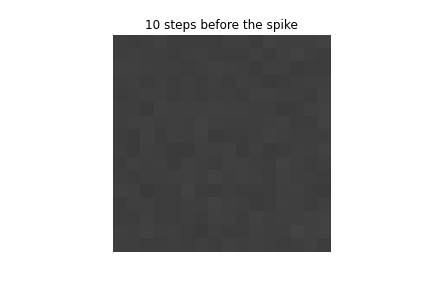
\includegraphics[width = 0.8\textwidth]{images/10.png}
    \caption{10 steps before the spike}
    %\label{fig:mesh1}
\end{figure}


\begin{figure}[h]
    \centering
    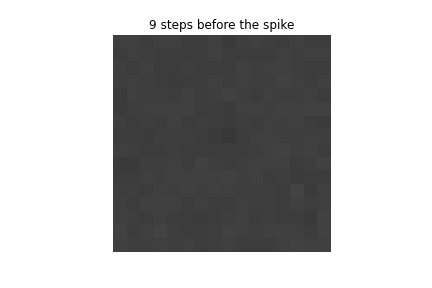
\includegraphics[width = 0.8\textwidth]{images/9.png}
    \caption{9 steps before the spike}
    %\label{fig:mesh1}
\end{figure}

\newpage
{\scshape EEE 482} \hfill {\scshape \large  Homework-\romannumeral2\relax} \hfill {\scshape Can Kocagil}
\smallskip
\hrule
\vspace{2mm}


\begin{figure}[h]
    \centering
    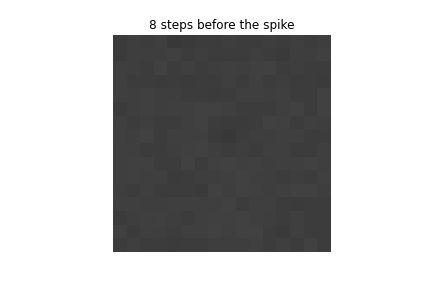
\includegraphics[width = 0.9\textwidth]{images/8.png}
    \caption{8 steps before the spike}
    %\label{fig:mesh1}
\end{figure}


\begin{figure}[h]
    \centering
    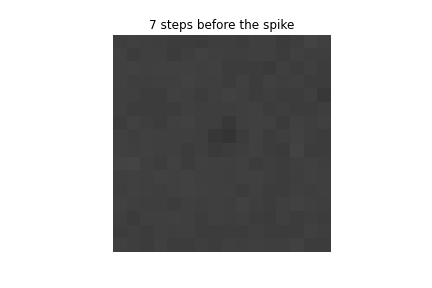
\includegraphics[width = 0.9\textwidth]{images/7.png}
    \caption{7 steps before the spike}
    %\label{fig:mesh1}
\end{figure}


\newpage
{\scshape EEE 482} \hfill {\scshape \large  Homework-\romannumeral2\relax} \hfill {\scshape Can Kocagil}
\smallskip
\hrule
\vspace{2mm}

\begin{figure}[h]
    \centering
    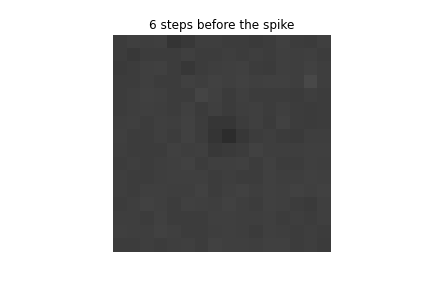
\includegraphics[width = 0.9\textwidth]{images/6.png}
    \caption{6 steps before the spike}
    %\label{fig:mesh1}
\end{figure}



\begin{figure}[h]
    \centering
    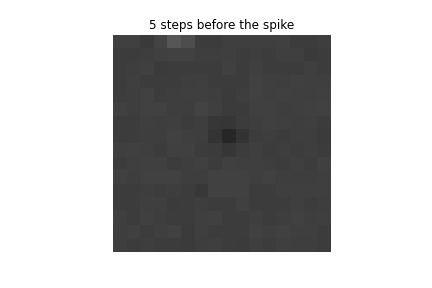
\includegraphics[width = 0.9\textwidth]{images/5.png}
    \caption{5 steps before the spike}
    %\label{fig:mesh1}
\end{figure}


\newpage
{\scshape EEE 482} \hfill {\scshape \large  Homework-\romannumeral2\relax} \hfill {\scshape Can Kocagil}
\smallskip
\hrule
\vspace{2mm}

\begin{figure}[h]
    \centering
    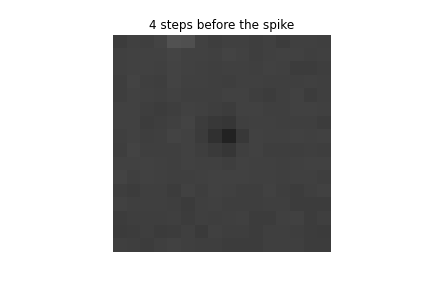
\includegraphics[width = 0.9\textwidth]{images/4.png}
    \caption{4 steps before the spike}
    %\label{fig:mesh1}
\end{figure}




\begin{figure}[h]
    \centering
    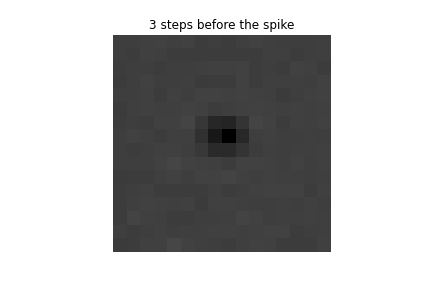
\includegraphics[width = 0.9\textwidth]{images/3.png}
    \caption{3 steps before the spike}
    %\label{fig:mesh1}
\end{figure}


\newpage
{\scshape EEE 482} \hfill {\scshape \large  Homework-\romannumeral2\relax} \hfill {\scshape Can Kocagil}
\smallskip
\hrule
\vspace{2mm}

\begin{figure}[h]
    \centering
    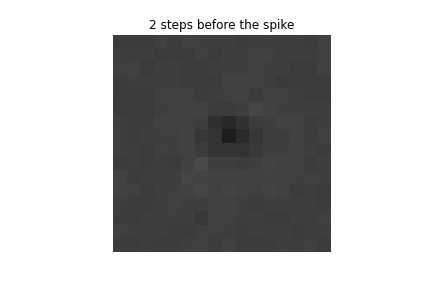
\includegraphics[width = 0.9\textwidth]{images/2.png}
    \caption{2 steps before the spike}
    %\label{fig:mesh1}
\end{figure}




\begin{figure}[h]
    \centering
    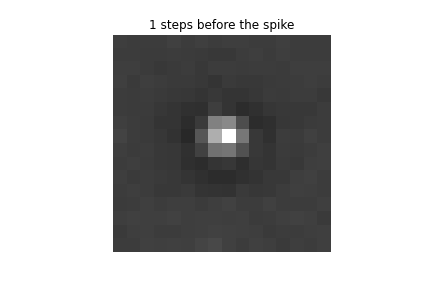
\includegraphics[width = 0.9\textwidth]{images/1.png}
    \caption{1 steps before the spike}
    %\label{fig:mesh1}
\end{figure}


\newpage
{\scshape EEE 482} \hfill {\scshape \large  Homework-\romannumeral2\relax} \hfill {\scshape Can Kocagil}
\smallskip
\hrule
\vspace{2mm}


From the derived STA filter, one can conclude that as we get closer to spike, the center region of the STA is become darkener until the last step before the spike. Then, the flash burst in the last step before the spike so that we can observe a clear \& distinct neural response. Hence, LGN cell is selective for gradual increase in darker regions until last step before spike and flash burst in last step before the spike under the assumption that STA model is linear receptive field. Additionally, by the analysis of stimulus and spike-train data, we can correlate the statistics of, i.e., mean and covariance, of the spatio-temporal distribution of stimuli corresponding to spike.


\subsection{Part B}

In the part b, we are asked to describe the changes in STA images across time by summing STA images over one of the spatial dimensions. Hence, we need to sum STA data in row and/or column wise. The following code snipped performs summation in both spatial dimensions and plot them side by side.

\begin{mintedbox}{python}
fig,axs = plt.subplots(1,2,figsize = (20,40)) 
axs[0].imshow(np.sum(sta,axis = 0),**kwargs)
axs[0].set_title(f"Row sum of STA")
axs[0].axis('off')
axs[1].imshow(np.sum(sta,axis = 1),**kwargs)
axs[1].set_title(f"Column sum of STA")
axs[1].axis('off')

plt.show()
\end{mintedbox}



\begin{figure}[h]
    \centering
    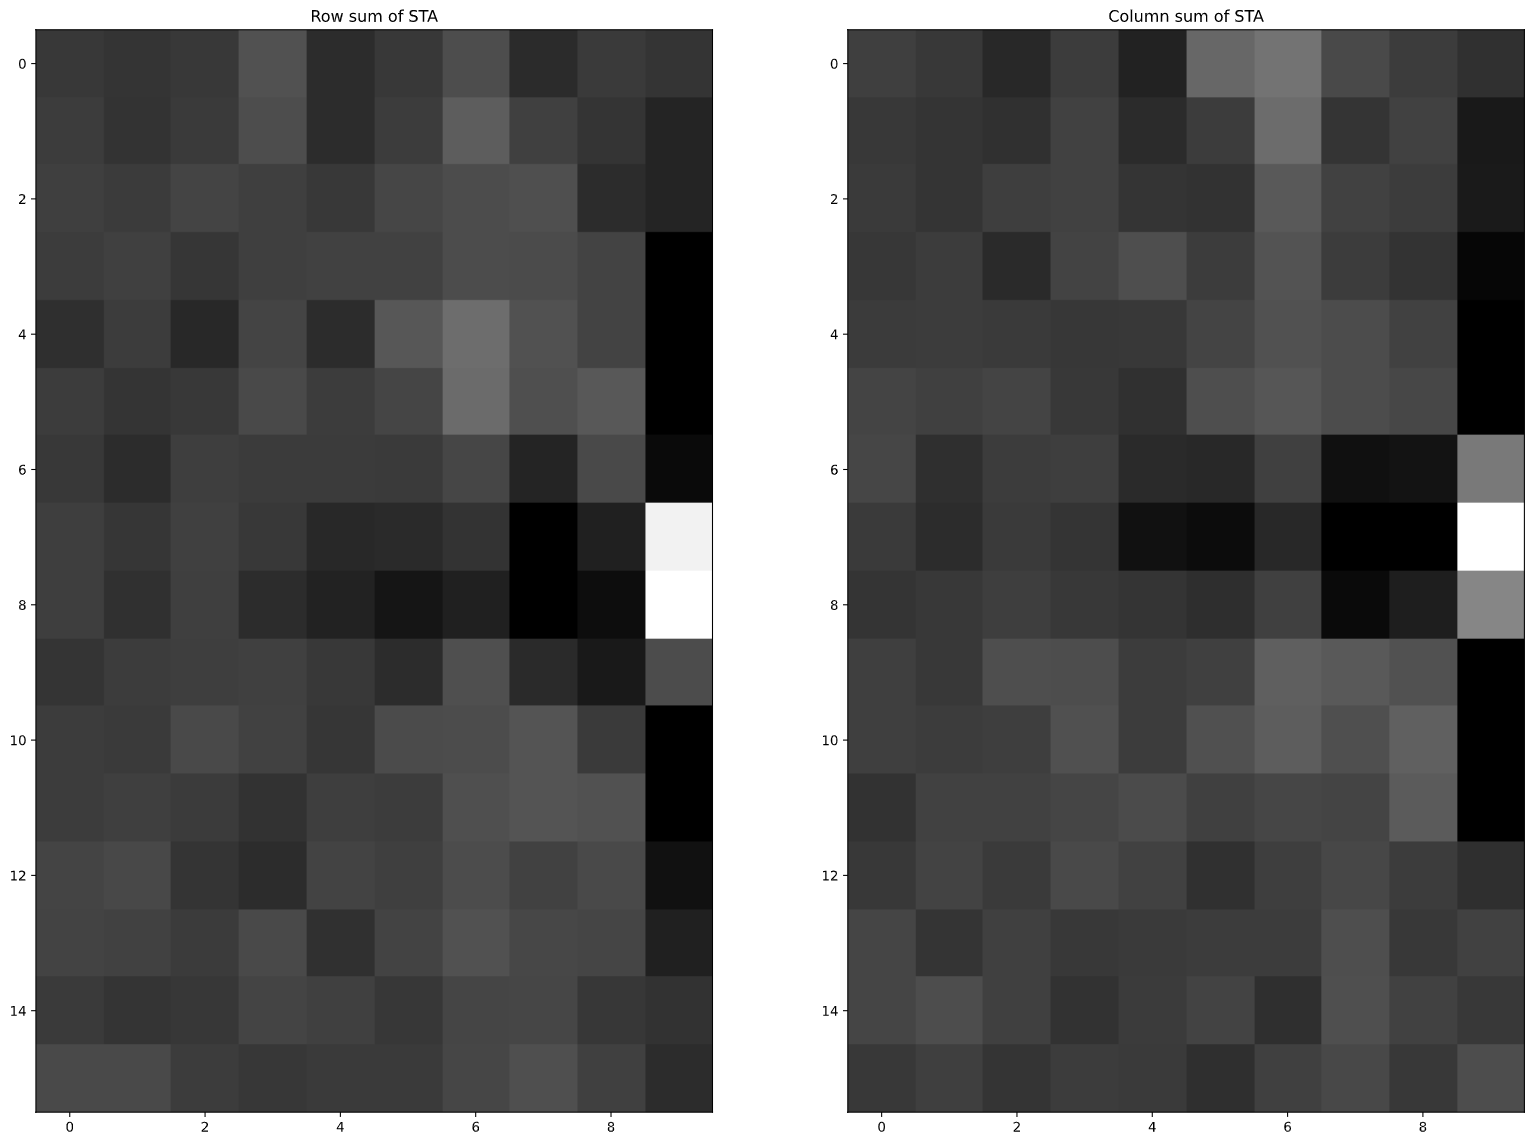
\includegraphics[width = 0.9\textwidth]{images/SpatialDimensionSummationofSTANew.png}
    \caption{Summation across spatial dimension (column\&row) wise respectively}
    %\label{fig:mesh1}
\end{figure}



\newpage
{\scshape EEE 482} \hfill {\scshape \large  Homework-\romannumeral2\relax} \hfill {\scshape Can Kocagil}
\smallskip
\hrule
\vspace{2mm}

The resulting images are in 16x10 format where absent 16 long spatial dimension is summed across the other spatial dimension. We can see from the above figure that row and column wise summation gives approximately symmetric distribution. As a clear distinction, as we get closer to left sides of the matrix (i.e., closer to spike regions) in time, comparatively, we can conclude that LGN cell is selective for a flash around pixel intensities 6-9. Additionally, one can conclude that the matrix is not space-time separable since the spikes solely depends on stimuli over time. Also, we can say that stimuli is not time-invariant (i.e., time-variant).


\subsection{Part C}

In this part of the question, we are asked to project the stimulus onto the STA image at a single time step prior to the spike and obtain the projection for each time sample by computing the Frobenius inner product between the stimulus image and the STA image.

\bigskip

Let's begin with the Frobenius inner product between the stimulus image and the STA image and how it performs. To be able compute, let's recall Frobenius inner product. Frobenius is basically inner product operation performs in matrix wise instead of vector wise. Note that Frobenius inner product is binary operation, i.e., returns a number, and denoted as follows

\begin{equation}
    \langle A,B \rangle_F = \sum_{i,j}^{}A_{ij} B_{ij}  \text{ where A \& B must have same dimension} 
\end{equation}

Here is the computation of Frobenius inner product between the stimulus image and the STA image followed by normalization is placed.

\begin{mintedbox}{python}
project_stim = np.array([np.sum(sta[:,:, num_timesteps - 1] * _stim) for _stim in np.swapaxes(stim,0,2)]) 
project_stim /= project_stim.max()
\end{mintedbox}


Hence, we succesfully computed the normalized version of Frobenius inner product between the stimulus image and the STA image. Let's look at the shape of the histogram lonely as a intuitive way of understanding the distribution of the projections.

\begin{mintedbox}{python}
kwargs = dict(
    bins=100, 
    alpha=.8,
    rwidth=.66,
   
)
plt.figure(figsize=(10, 5))
plt.hist(project_stim,color='g', **kwargs)
plt.title('Histogram of Stimilus Projections on STA')
plt.ylabel('Spike Frequency')
plt.xlabel('Normalized Stimulus Projection')
plt.show()
\end{mintedbox}

\newpage
{\scshape EEE 482} \hfill {\scshape \large  Homework-\romannumeral2\relax} \hfill {\scshape Can Kocagil}
\smallskip
\hrule
\vspace{2mm}

\begin{figure}[h]
    \centering
    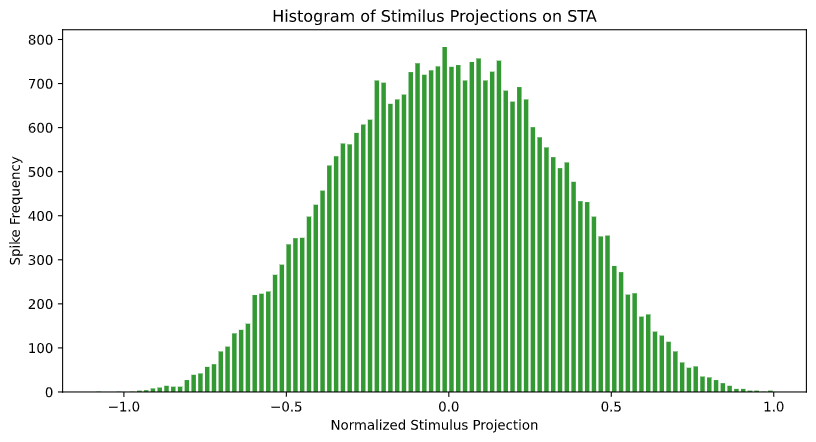
\includegraphics[width = 0.9\textwidth]{images/HistogramSTA.png}
    \caption{Histogram of normalized stimulus projections}
    %\label{fig:mesh1}
\end{figure}

Then, the next step is to create histogram for stimulus projections at time bins where a non-zero spike count was observed. To do that, I find the indexes of non-zero spikes followed by Frobenius inner product between the stimulus image and the STA image. Here is the code for computation of stimulus projections at time bins where a non-zero spike count was observed.

\begin{mintedbox}{python}
spike_times = counts.nonzero()[0]

project_stim_nonzero = np.array([np.sum(sta[:,:, num_timesteps - 1] * stim[:,:,i]) for i in spike_times]) 
project_stim_nonzero /= project_stim_nonzero.max()
\end{mintedbox}

As a prior step to plot both histograms on top of each other, let's look at the distribution of non-zero spikes normalized stimulus projections as follows.

\begin{mintedbox}{python}
plt.figure(figsize=(10, 5))
plt.hist(project_stim_nonzero, **kwargs,color='orange')
plt.title('Histogram of Stimilus Projections on STA for non-zero spikes')
plt.ylabel('Spike Frequency')
plt.xlabel('Normalized Stimulus Projection')
plt.show()
\end{mintedbox}


\newpage
{\scshape EEE 482} \hfill {\scshape \large  Homework-\romannumeral2\relax} \hfill {\scshape Can Kocagil}
\smallskip
\hrule
\vspace{2mm}

\begin{figure}[h]
    \centering
    \includegraphics[width = 0.9\textwidth]{images/NZ_HİST.png}
    \caption{Histogram of Stimulus Projections on STA for non-zero spikes}
    %\label{fig:mesh1}
\end{figure}


Then, the final step is to plot both histograms on top of each other to see whether STA significantly discriminates spike-eliciting stimuli or not. So, let's plot both histograms on top of each other.


\begin{mintedbox}{python}
plt.figure(figsize=(10, 5))
plt.hist(project_stim, **kwargs)
plt.title('Comparison Histogram of Stimilus Projections on STA')
plt.hist(project_stim_nonzero, **kwargs)
plt.ylabel('Spike Frequency')
plt.xlabel('Normalized Stimulus Projection')
plt.legend(['For all Spikes','For nonzero spikes'])
plt.show()
\end{mintedbox}


\begin{figure}[h]
    \centering
    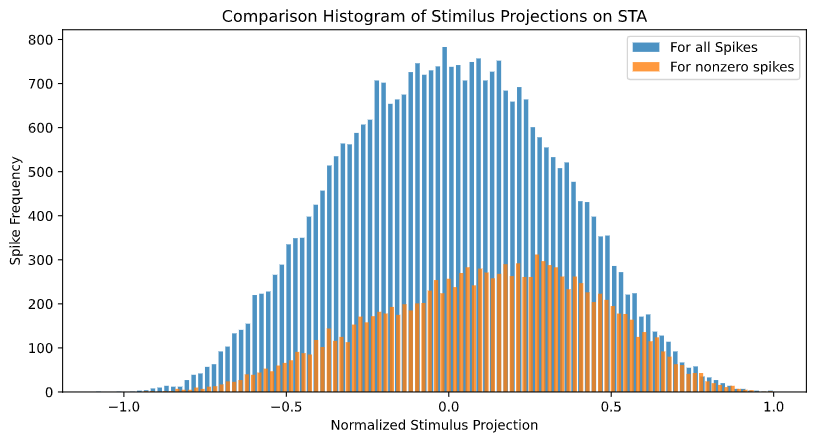
\includegraphics[width = 0.8\textwidth]{images/comparisonhist.png}
    \caption{Comparison Histogram of Stimulus Projections on STA}
    %\label{fig:mesh1}
\end{figure}



\newpage
{\scshape EEE 482} \hfill {\scshape \large  Homework-\romannumeral2\relax} \hfill {\scshape Can Kocagil}
\smallskip
\hrule
\vspace{2mm}

As we can see from the FIGURE 14, the distribution of stimulus projections on STA images for all spikes are bringing to mind the centered (i.e., $\mu = 0$) Gaussian (Normal) distribution whereas the distribution of stimulus projections on STA images for non-zero spikes are reminding the  Gaussian distribution where mean $\mu$ is in between $[0.2,0.4]$. Since the shape of the distribution can fit into Gaussian line, we can say much about the both projections. Finally, strictly speaking, STA discriminates the spike-eliciting stimuli significantly since the projections of the stimulus onto the STA image with non-zero spikes turn centered Gaussian distribution into Gaussian with mean shifted version. Consequently, we can easily say that STA significantly discriminates spike-eliciting stimuli.


\section{Question 2}

In this question, we are going to generate receptive fields and their responses of each neuron to given image \textbf{hw2\_image.bmp} in a computational manner.


\subsection{Part A}
In this part, we are going to construct an on-center Difference-of-Gaussian's (DOG) center-surround receptive field centered at 0 as follows

\begin{equation}
    D(x,y) = \frac{1}{2 \pi \sigma_c^2} e^{(-x^2 + y^2)/2 \sigma_c^2} - \frac{1}{2 \pi \sigma_s^2} e^{(-x^2 + y^2)/2 \sigma_s^2}
\end{equation}


\vspace{2mm}

In the context of imaging, Difference of Gaussians (DoG) is a feature enhancement algorithm that involves the subtraction of one Gaussian blurred version of an original image from another, less blurred version of the original \cite{enwiki:1007271206}. In the simple case of grayscale images, the blurred images are obtained by convolving the original grayscale images with Gaussian kernels having differing width (standard deviations)\cite{enwiki:1007271206}. Hence, it is a classical 2-D image convolution operation (actually, it is cross-correlation) with DoG kernel. As a further information, blurring an image using a Gaussian kernel suppresses only high-frequency spatial information whereas subtracting one image from the other preserves spatial information that lies between the range of frequencies that are preserved in the two blurred images\cite{enwiki:1007271206}. This is one of most significant property of DoG. Thus, the DoG is a spatial band-pass filter that attenuates frequencies in the original grayscale image that are far from the band center in 2-D domain. \cite{enwiki:1007271206}.

\bigskip

In our case, we will use the DoG as a 2-D filter to detect edges of source image. As we previously talked about the DoG applications on feature enhancement, it is powerful method to identify edges of the foreground objects. Furthermore, DoG filtering is very useful method in reduction of Gaussian noise that is generally active in higher spatial frequencies. Some classical filtering operations are sensitive to Gaussian noise in high spatial frequency so that they tend to enhance Gaussian noise while enhancing the features of foreground object. Hence, DoG is desirable algorithm when it comes to reducing the high frequency noises, it's the reason why DoG is preferable for vision problems with higher degree of Gaussian noise. So, let's generate 21x21 DoG receptive field with $\sigma_c = 2$ and $\sigma_s = 4$ and display in both 2-D \& 3-D surface to understand the kernel in a visual way. Here is the Python code for generating DoG receptive field with given $\sigma_c = 2$ , $\sigma_s = 4$ and size = (21x21).

\newpage
{\scshape EEE 482} \hfill {\scshape \large  Homework-\romannumeral2\relax} \hfill {\scshape Can Kocagil}
\smallskip
\hrule
\vspace{2mm}

\begin{mintedbox}{python}
def DoG_Receptive_Field(std_c:int,std_s:int,size:int) -> np.ndarray:
    """
        Construct an on-center difference-of-gaussians (DoG) center-surround receptive field    centered at 0 with the given size. Generally, the Difference of Gaussian module is a   filter that  identifies edges.Additionally, DoG is a feature enhancement algorithm that involves the subtraction of one Gaussian blurred version of an original image from another, less blurred version of the original

            Arguments:
                - std_c (int) : Standard deviation of lower sigma
                - std_s (int) : Standard deviation of higher sigma
                - size  (int) : Size of DoG kernel

            Returns:
               - DoG_kernel (np.ndarray) : DoG kernel with given (size,size)

    """

    import math
    
    # Computing lower sigma kernel:
    low_sigma_kernel  = np.fromfunction(
        lambda x, y: (1/(2*math.pi*std_c**2)) * math.e ** ((-1*((x-(size-1)/2)** 2+(y-(size-1)/2)**2))/(2*std_c**2)), (size, size)        
        )

    # Computing higher sigma kernel:
    high_sigma_kernel = np.fromfunction(
        lambda x, y: (1/(2*math.pi*std_s**2)) * math.e ** ((-1*((x-(size-1)/2)**2+(y-(size-1)/2)**2))/(2*std_s**2)), (size, size)
        )

    # DoG kernel:
    DoG_kernel = low_sigma_kernel - high_sigma_kernel

    return DoG_kernel
\end{mintedbox}

Here, we successfully generate a function that gives DoG receptive field with any size and $\sigma$. Then, let's sample a 21x21 receptive field as follows

\begin{mintedbox}{python}
DoG_kernel = DoG_Receptive_Field(**
dict(
    size = 21,
    std_c = 2,
    std_s = 4

))
\end{mintedbox}


\newpage
{\scshape EEE 482} \hfill {\scshape \large  Homework-\romannumeral2\relax} \hfill {\scshape Can Kocagil}
\smallskip
\hrule
\vspace{2mm}

Then, let's display the DoG kernel on both 2-D and 3-D surface as follows. Note that generic 2-D and 3-D filter plotting functions are written to be used in later parts of the question. The code for plotting filters will be only displayed below, and will be using just by calling the function when necessary. Hence, let's see the visualization of DoG filters. The first code snipped is for plotting the kernel on 2-D surface whereas the second one stands for 3-D filter visualization. 

\begin{mintedbox}{python}
def plotFilter2D(kernel:np.ndarray,title:str,
                 cmap:str='coolwarm',
                 figsize:tuple = (10,10),
                 kwargs:dict = None) -> None:

    """
        Given the kernel, plot the kernel in 2-D surface.

            Arguments:
                - kernel (np.ndarray) : Kernel to be plotted
                - title  (str)        : Title of the figure
                - cmap   (str)        : Texture of the figure
                - figsize (tuple)     : Figure size
                - kwargs (dict)       : Additional arguments to plot if exists

            Returns:
                - None

    """

    plt.figure(figsize = figsize)

    if kwargs is not None:
        plt.imshow(kernel,cmap=cmap,**kwargs)
    else:
        plt.imshow(kernel,cmap=cmap)       
    
    plt.title(title)
    plt.colorbar()
    plt.show()
\end{mintedbox}

Then, here is the code for 3-D filter visualization.


\begin{mintedbox}{python}
def plotFilter3D(kernel:np.ndarray,title:str,
                 kernel_name:str, 
                 cmap:str='coolwarm',
                 figsize:tuple = (10,10),
                 kwargs:dict = None) -> None:

    """
        Given the kernel, plot the kernel in 2-D surface.

            Arguments:
                - kernel (np.ndarray) : Kernel to be plotted
                - title  (str)        : Title of the figure
                - kernel_name (str)   : The name of the filter/kernel
                - cmap   (str)        : Texture of the figure
                - figsize (tuple)     : Figure size
                - kwargs (dict)       : Additional orguments to plot if exists

            Returns:
                - None

    """

    fig_3D = plt.figure(figsize = (10,10))
    size = kernel.shape[0]
    ax_3D = plt.axes(projection='3d')
    x,y = np.meshgrid(
        np.arange( - int(size / 2), 1 + int(size / 2)),
        np.arange( - int(size / 2), 1 + int(size / 2))
                )
    
    if kwargs is not None:
        ax_3D.plot_surface(x, y, kernel,cmap = cmap, **kwargs)
    else:
        ax_3D.plot_surface(x, y,kernel, cmap = cmap)   
    
    ax_3D.set_xlabel('x')
    ax_3D.set_ylabel('y')
    ax_3D.set_zlabel(f'{kernel_name}(x, y)')
    plt.title(title)
    plt.show()
\end{mintedbox}

Finally, we can plot the DoG filter with the parameters $\sigma_c = 2$ , $\sigma_s = 4$ and size = (21x21).

\begin{mintedbox}{python}
kwargs = dict(
    rstride=1,
    cstride=1,     
    edgecolor='none'
)

plotFilter2D(DoG_kernel,f'Difference of Gaussian (DoG) kernel with Stds {(2,4)} in 21x21 form')

plotFilter3D(DoG_kernel,f'Difference of Gaussian (DoG) kernel with Stds {(2,4)} in 21x21 form','DoG', kwargs = kwargs)
\end{mintedbox}



\newpage
{\scshape EEE 482} \hfill {\scshape \large  Homework-\romannumeral2\relax} \hfill {\scshape Can Kocagil}
\smallskip
\hrule
\vspace{2mm}

\begin{figure}[h]
    \centering
    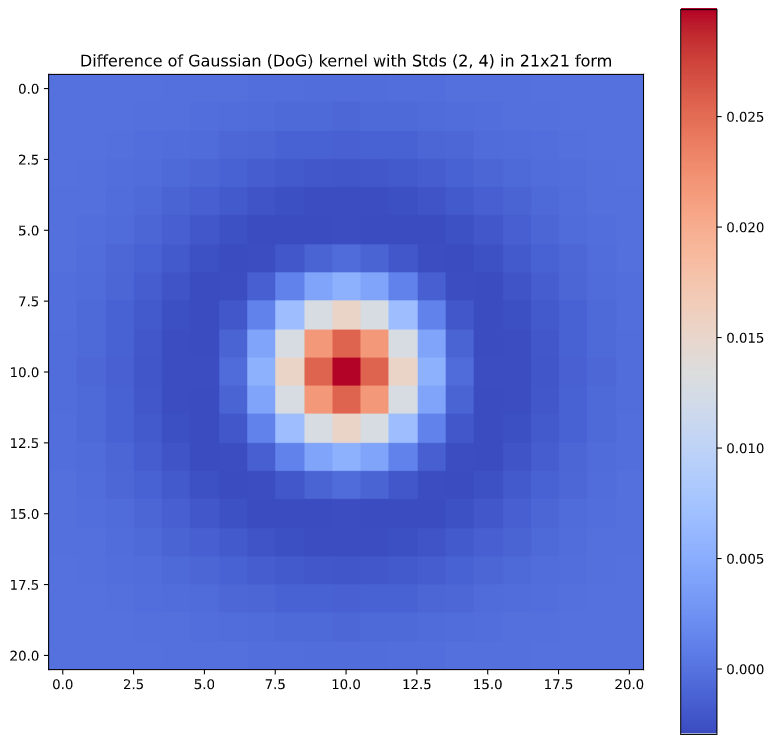
\includegraphics[width = 0.6\textwidth]{images/DoG2d.png}
    \caption{Difference of Gaussian (DoG) kernel with Stds {(2,4)} in 21x21 form}
    %\label{fig:mesh1}
\end{figure}

3-D visualization of Gaussian based kernels are better way to get insights from the distributions. So, here I plotted our 21x21 DoG kernel in 3-D canvas.

\begin{figure}[h]
    \centering
    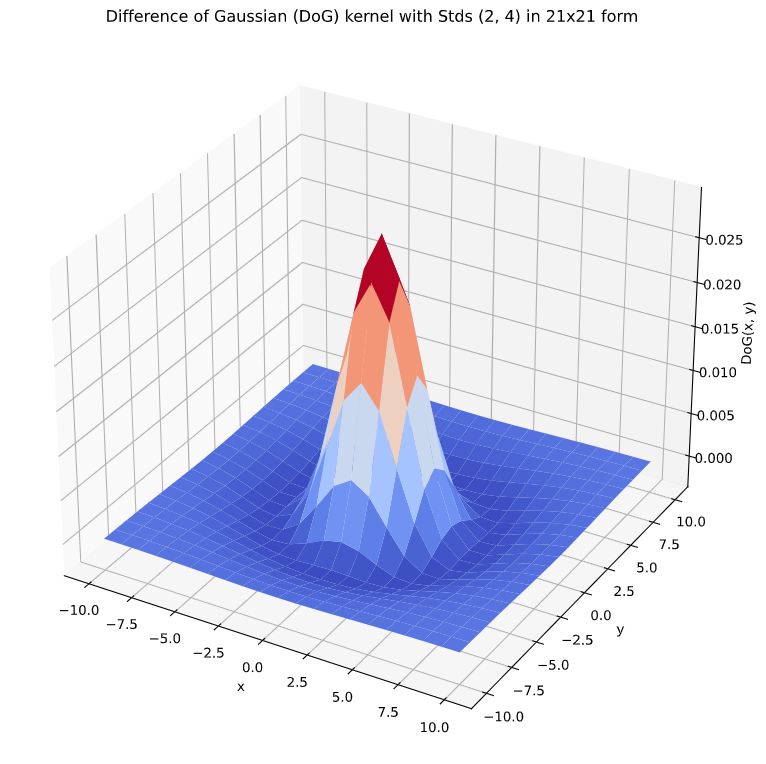
\includegraphics[width = 0.6\textwidth]{images/DoG3d.png}
    \caption{Difference of Gaussian (DoG) kernel with Stds {(2,4)} in 21x21 form}
    %\label{fig:mesh1}
\end{figure}

\subsection{Part B}
In this part of the question, we are assuming that there is a separate LGN neuron with a receptive field centered on each pixel in the image with the knowledge that neurons in lateral geniculate nuclei (LGN) have DOG receptive fields. So, here we are going to compute the responses of each neuron to the image given in \textbf{hw2\_image.bmp}.


\bigskip

As a prior step along the computation of responses of each neuron to given image, let's visualize the given image as follows.


\begin{mintedbox}{python}
image = plt.imread('hw2_image.bmp')
plt.figure(figsize=(10,10))
plt.imshow(image)
plt.axis('off')
plt.show()
\end{mintedbox}

\begin{figure}[h]
    \centering
    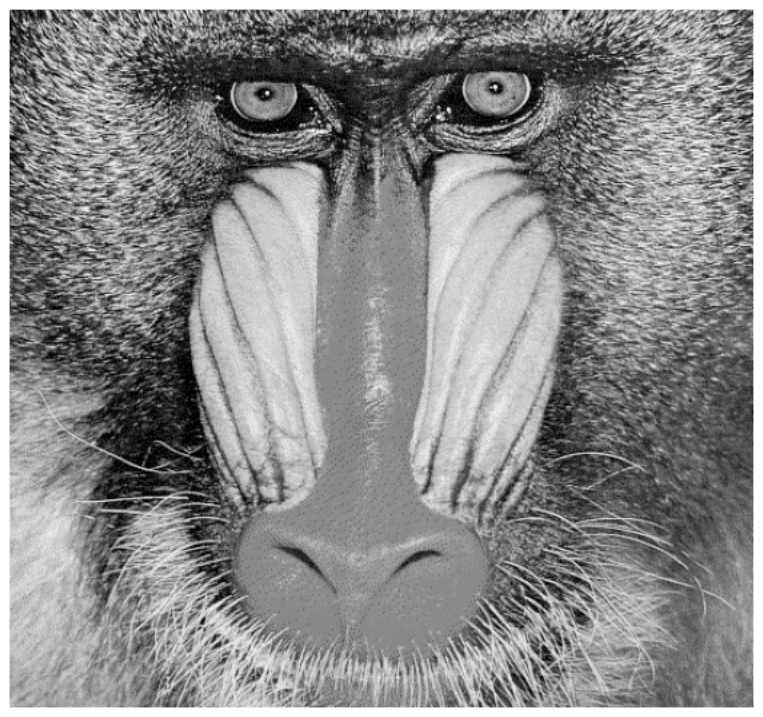
\includegraphics[width = 0.6\textwidth]{images/image.png}
    \caption{Given input image}
    %\label{fig:mesh1}
\end{figure}

To be able to compute the responses of each neuron to the image given in \textbf{hw2\_image.bmp}, we need to create sliding window over the image such DoG receptive field kernel can moves along the spatial dimensions of the input image. In the context of computational neuroscience, the activity of an LGN cell can be explained as the amount of overlap between DoG receptive field and its input. In mathematics domain, this process is called \textbf{convolution}. 2-D  Convolution is performed by multiplying and accumulating the instantaneous values of the overlapping samples corresponding to input images and its filter. So, let's create a convolution function as follows. But, as a prior step to create convolution function, we need to have sliding window over the padded image (Zero padding for \textbf{'same'} convolution operation, i.e., pad the image so that resulting image have the same spatial dimensions as before). Let's see the Python code for sliding window.

\newpage
{\scshape EEE 482} \hfill {\scshape \large  Homework-\romannumeral2\relax} \hfill {\scshape Can Kocagil}
\smallskip
\hrule
\vspace{2mm}

\begin{mintedbox}{python}
class _Window(object):
  """
    This class creates a generator that slide over the given image with
    predefined step and window size.

      Attributes:
        - image      : input image to be sliding
        - step_size  : it determines how much slice the generator extract
        - dims       : resulting image's dimensions

      Methods:
        - __iter__   : creates a generator over the image with given patch dimensions

  """
  def __init__(self,image : np.ndarray, step_size:tuple, dims: tuple):
    """ 
      Creates an constructor for _Window class, this method encapsulates
      all necessary data to generate windows over image.  

    """
    self.image = image 
    self.dims = dims 
    self.step_size = step_size

  def __iter__(self):
    """ Generator function to window over image. """
    for x in range(self.dims[0]):
      for y in range(self.dims[1]):
        yield self.image[x:x + self.step_size[0], y:y + self.step_size[1]]
\end{mintedbox}

Hence, all we need to do is to pad the image with zeros if necessary, then multiply the corresponding entries of image patches with DoG kernel, then accumulate the resulting multiplication to see fill the corresponding entry of convolved image. Here is the Python code for convolution.


\begin{mintedbox}{python}
def Conv2D(source_image : np.ndarray, kernel: np.ndarray) -> np.ndarray:
  """
   Convolution is the process of adding each element of the image to its local neighbors,weighted by the kernel. This is related to a form of mathematical convolution.
   
      Arguments:
        - source_image   (np.ndarray) : Gray scale image to be convolved
        - kernel         (np.ndarray) : Kernel to be sliding over the image

      Returns:
        - conv_image     (np.ndarray) : Resulting convolved image
  """

  assert (len(source_image.shape)   == 2), "Image is not gray scale" 
  assert (len(kernel.shape) == 2), "Kernel is not in required size"      
  
  source_image =  np.asarray(source_image).clip(0,255).copy()
  H,W = source_image.shape
  k_h,k_w = kernel.shape
  padded_image = np.pad(array = source_image, pad_width = max(k_w,k_w) // 2 + 1, mode = 'constant')

  new_H,new_W = padded_image.shape
  h_pad , w_pad  =  (new_H - H) , (new_W - W)

  # Creating sliding window:
  image_window = _Window(padded_image,(k_h,k_w),(new_H - h_pad, new_W - w_pad))

  #kernel = np.flipud(np.fliplr(kernel))
  # Main operation:
  conv_image = [(patch * kernel).sum() for patch in image_window]
  
  return np.array(conv_image).reshape(H,W)
\end{mintedbox}

Finally, we can compute the responses of each neuron to the given image. Note that even the given image has 3 channels, it is actually replica of 1 channel so that any random channel can be slicing as a source image for the following computations.

\begin{mintedbox}{python}
gray_image = image[:,:,0]
filtered_image = Conv2D(gray_image,DoG_kernel)

plt.figure(figsize=(7,7))
plt.imshow(min_max_scaler(filtered_image),cmap = 'gray')
plt.title('Convolved image by DoG kernel')
plt.axis('off')
plt.show()
\end{mintedbox}


\begin{figure}[h]
    \centering
    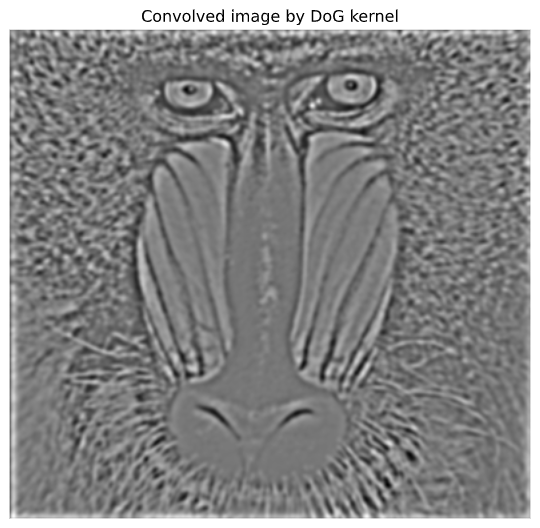
\includegraphics[width = 0.6\textwidth]{images/CONV_image.png}
    \caption{Convolved image with DoG receptive field.}
    %\label{fig:mesh1}
\end{figure}


\newpage
{\scshape EEE 482} \hfill {\scshape \large  Homework-\romannumeral2\relax} \hfill {\scshape Can Kocagil}
\smallskip
\hrule
\vspace{2mm}

Note that MIN-MAX scaling operation is applied on resulting image to plot in matplotlib's input format, i.e., the pixel intensities should be in the range 0-1 or 0-255. It has no functionality other than that in our case. Just be concrete on the discussion, let's provide the code for MIN-MAX scaler.

\begin{mintedbox}{python}
def min_max_scaler(matrix : np.ndarray)-> np.ndarray :
  """
    Given the matrix, apply normalization as follow:

        norm_matrix = (matrix - min_val) / (max_val - min_val)

    Arguments:
      -  matrix     (np.ndarray) : Input Matrix

    Returns:
      - norm_matrix (np.ndarray) : Normalized version of matr

  """
  matrix = np.asarray(matrix).copy()
  max_val = matrix.max()
  min_val = matrix.min()

  return (matrix - min_val) / (max_val - min_val)
\end{mintedbox}


\subsection{Part C}

In this part of the question, we are asked to build an edge detector by thresholding the neural activity image (i.e., setting all values above a certain threshold to 1 and the remainder to 0.). Hence, we need to find a optimal threshold value so that we can identifies edges in distinct way. To do that, one can approach different methods such as manual thresholding, i.e., trial-and-error fashion, or we can use automatic thresholding algorithms such as Otsu method. Otsu's automatic thresholding is a method that separates background and foreground of image with automatically computed threshold value. This  threshold is computed via minimizing the within-class variance or  maximizing the inter-class variability that yields same result. However, note that computing threshold value by maximizing the inter-class variance is more computationally efficient method. Hence, I created a Otsu thresholding method for finding automatic threshold value of the given source image. Here is the code for Otsu thresholding.

\begin{mintedbox}{python}
def otsu_threshold(source_image: np.ndarray) -> np.ndarray:
    """
    Otsu's automatic thresholding method that seperates background and foreground of image with automatically computed threshold value. This threshold is computed via minimizing the within-class variance or maximizing the inter-class variability that yields same results. However, note that computed threshold value by maximizing the inter-class variance is more computationally efficient method. 

      Arguments:
        - source_image (np.ndarray) : Source image to be thresholded by Otsu

      Returns:
        - thres_image  (np.ndarray) : Resulting image after applying Otsu's method

  """

    assert (len(source_image.shape) == 2), "Image is not gray scale"     
    
    source_image =  np.asarray(source_image).clip(0,255).copy()

    hist =  [np.sum(pixel == source_image) for pixel in np.arange(256)]

    
    otsu_thres = 0
    var = 0
    max_val = 256
    
    for thres in np.arange(256):

      # For first class, mean and variance:
      w_0 = sum(pixel for pixel in hist[:thres])
      mu_0 = sum([i * hist[i] for i in range(thres)]) / w_0 if w_0 > 0 else 0   

      # For second class, mean and variance:
      w_1 = sum(pixel for pixel in hist[thres:])          
      mu_1 = sum([j * hist[j] for j in range(thres, max_val)]) / w_1 if w_1 > 0 else 0

      # calculating inter-class variance         
      s = w_0 * w_1 * (mu_0 - mu_1) ** 2

      # Set threshold if new inter class variance is bigger than previous
      otsu_thres = thres - 1 if s > var else otsu_thres
      var = s if s > var else var

    #print(f'Self written Otsu threshold value is {otsu_thres}')  

    # Apply thresholding: Hence
    source_image[source_image >= otsu_thres] = 255
    source_image[source_image < otsu_thres] = 0

    return source_image.astype(np.uint8)
\end{mintedbox}

As we discuss, Otsu thresholding is automatic way of thresholding that is desirable for autonomous tasks. Additionally, Otsu thresholding performs good if calculated histogram comes from the bimodal distribution (having two different modes, clear \& distinctive local peaks, etc.). Eventually, Otsu method will find proper value of thresholding that successfully separates background from foreground if tonal distribution of the image comes from the bimodal distribution. Hence, performance of Otsu method is limited. Therefore, it is not always good idea to apply Otsu thresholding before having a idea of tonal distribution of images. In a nutshell, it is always good idea to tune the threshold value in hand-crafted way so I also create a function that separates the background from the foreground in manual way.

\newpage
{\scshape EEE 482} \hfill {\scshape \large  Homework-\romannumeral2\relax} \hfill {\scshape Can Kocagil}
\smallskip
\hrule
\vspace{2mm}


\begin{mintedbox}{python}
def manuel_thresholding(source_image: np.ndarray,threshold:int) -> np.ndarray:
    """
        Given the source image and threshold, apply thresholding (i.e., setting all values above a certain threshold to 1 and the remainder to 0.

            Arguments:
                - source_image (np.ndarray) : Source image to be thresholded
                - threshold    (int)        : Threshold value

            Returns:   
                - thres_image  (np.ndarray) : Resulting image after applying threshold

    """

    
    assert (len(source_image.shape) == 2), "Image is not gray scale"     
    
    source_image =  np.asarray(source_image).clip(0,255).copy()

    # Apply thresholding:
    source_image[source_image >= threshold] = 255
    source_image[source_image < threshold] = 0

    return source_image.astype(np.uint8)
\end{mintedbox}

Now, we can see the edge detector's performance so let's plot the resulting images after both manual and Otsu thresholding method. Note that I applied MIN-MAX scaling operation on filtered images since the output of the convolution operation results the pixel intensity values in range $[-50,50]$. By doing that, I transformed the pixel values into range $[0,255]$ as 8-bit integers. So, we can pass the resulting image into both Otsu and manual thresholding to see the edge detector's performance.

\begin{mintedbox}{python}
img = np.array(min_max_scaler(filtered_image) * 255, dtype = np.uint8)
plt.figure(figsize=(7,7))
plt.imshow(otsu_threshold(img),cmap = 'gray')
plt.title('Convolved image by DoG kernel')
plt.axis('off')
plt.show()

plt.figure(figsize=(7,7))
plt.imshow(manuel_thresholding(img,115),cmap = 'gray')
plt.title('Convolved image by DoG kernel')
plt.axis('off')
plt.show()
\end{mintedbox}


\newpage
{\scshape EEE 482} \hfill {\scshape \large  Homework-\romannumeral2\relax} \hfill {\scshape Can Kocagil}
\smallskip
\hrule
\vspace{2mm}


\begin{figure}[h]
    \centering
    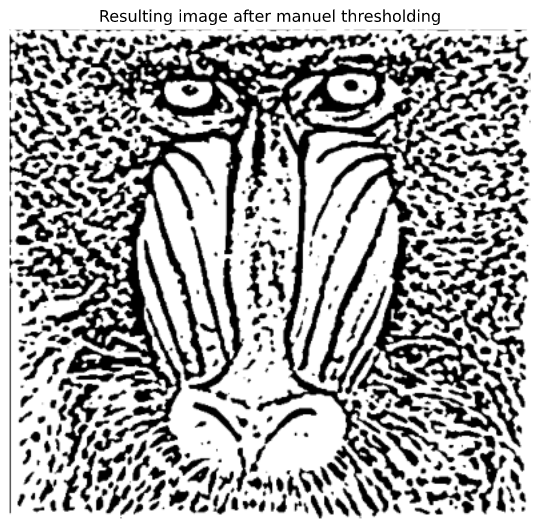
\includegraphics[width = 0.6\textwidth]{images/maneul_ths.png}
    \caption{Resulting image after manual thresholding}
    %\label{fig:mesh1}
\end{figure}


\begin{figure}[h]
    \centering
    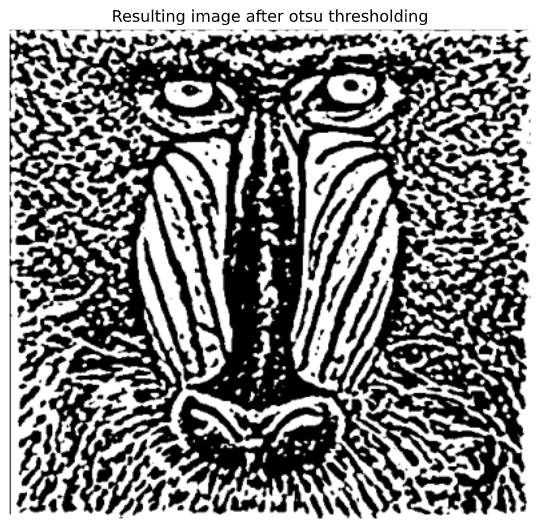
\includegraphics[width = 0.6\textwidth]{images/otsul_ths.png}
    \caption{Resulting image after otsu thresholding}
    %\label{fig:mesh1}
\end{figure}

\newpage
{\scshape EEE 482} \hfill {\scshape \large  Homework-\romannumeral2\relax} \hfill {\scshape Can Kocagil}
\smallskip
\hrule
\vspace{2mm}

As we can see from the figures, we successfully identifies the edges of the foreground object. In manual thresholding case with the threshold value 115, we detect smoother edges compared to Otsu case. In otsu binarization, we see that even we identifies a edges of the object, the contour of the foreground is also visible so that manual thresholding gives better edge performance in this case. Additionally, we can say that Otsu's binarization is approximately dilated version of the manual thresholding.

\subsection{Part D}

In this part, as similar to part A, we are asked to construct receptive field with 21x21 form but in this case, the distribution of the receptive field comes from the Gabor. Mathematically, we can represent the Gabor kernel as follows


\begin{equation}
    D(\vec{x}^{\,}) = \exp{\left(- (\vec{k}^{\,}(\theta) \cdot \vec{x}^{\,})^2 / 2\sigma_l^2 - (\vec{k_\bot}^{\,}(\theta) \cdot \vec{x}^{\,})^2 / 2\sigma_w^2 \right)} \cos{\left(2\pi \frac{\vec{k_\bot}^{\,}(\theta) \cdot \vec{x}^{\,}}{\lambda} + \phi \right)}
\end{equation}

Here $\vec{k_\bot}^{\,}(\theta)$ and $\theta$ is a unit vector with the orientation $\theta$,  $\vec{k_\bot}^{\,}(\theta)$ is a unit vector orthogonal to $\vec{k_\bot}^{\,}(\theta)$ and $\theta, \sigma_l,\sigma_w,\lambda$ and $\phi$ are parameters of the Gabor kernel. As provided, we have $\theta$ = $\pi/2$, $\sigma_l = \sigma_w$ = 3, $\lambda$ = 6, and $\phi$ = 0. So, let's begin with the discussion of the Gabor filter and its applications to our case. Gabor is a linear filter used for texture analysis, edge detection, feature extraction, etc. which essentially means that it analyzes whether there is any specific frequency content in the image in specific directions in a localized region around the point or region of analysis\cite{enwiki:993157632}. Frequency and orientation representations of Gabor filters are claimed by many contemporary vision scientists to be similar to those of the human visual system \cite{enwiki:993157632} as we are computing responses of each neuron to the given image. Hence, the visual cortex of some mammals can be expressed by these filters. As we discuss, Gabor filter considers the optimal localization properties in both spatial \& frequency domain with orientations so that they are useful in egde detection, segmentation problems. We can consider Gabor filters as a sinusoidal oriented 2-D Gaussian filters that considers the spatial neighborhoods in cross-correlations. Let's see a figure of Gabor filter as a intuitive way of understanding the internal structure.


\begin{figure}[ht]
    \centering
    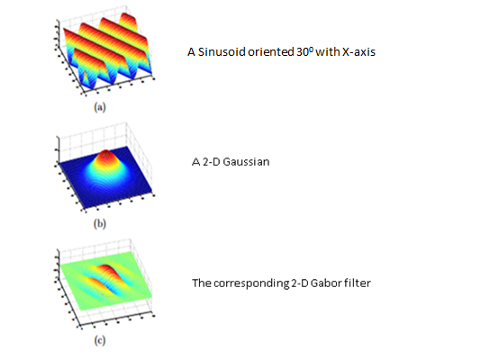
\includegraphics[width = 0.75\textwidth]{images/Gabor.png}
    \caption{A 2-D Gabor filter obtained by modulating the sine wave with a Gaussian}
    %\label{fig:mesh1}
\end{figure}

\newpage
{\scshape EEE 482} \hfill {\scshape \large  Homework-\romannumeral2\relax} \hfill {\scshape Can Kocagil}
\smallskip
\hrule
\vspace{2mm}

As we can see from the figure, sinusoidal component of Gabor filters is spatially localized. Intuitively, we can use different orientation of 2-D Gabor filters to extract spatially meaningful features from the images. Then, we can move to construction of Gabor receptive fields as follows.



\begin{mintedbox}{python}
def Gabor_Receptive_Field(std_l:int,std_w:int,
                          theta:float,Lambda:int,
                          psi:int, size:tuple) -> np.ndarray:
    """
        Gabor Receptive Field is a linear filter used for texture analysis, which essentially            means that it analyzes whether there is any specific frequency content in the image in           specific directions in a localized region around the point or region of analysis
        
            Arguments:
                - std_l  (int)   : Standard deviation of lower sigma
                - std_w  (int)   : Standard deviation of higher sigma                
                - theta  (float) : Orientation
                - Lambda (int)   : Gabor filter parameter 
                - psi    (int)   : Gabor filter parameter
                - size   (tuple) : Size of Gabor kernel

            Returns:
               - Gabor_kernel (np.ndarray) : Gabor kernel with given (size,size)

    """


    import math

    x, y = np.meshgrid(np.arange(- int(size[0] / 2), 1 + int(size[0] / 2)),
                       np.arange(- int(size[1] / 2), 1 + int(size[1] / 2)))


    # Rotation
    x_theta = x * np.cos(theta) + y * np.sin(theta)
    y_theta = -x * np.sin(theta) + y * np.cos(theta)

    # Main function for creating Gabor filter:
    Gabor_kernel = np.exp(-.5 * (x_theta ** 2 / std_l ** 2 + y_theta ** 2 / std_w ** 2)) * np.cos(2 * np.pi / Lambda * x_theta + psi)


    return Gabor_kernel
\end{mintedbox}

As provided, we have $\theta$ = $\pi/2$, $\sigma_l = \sigma_w$ = 3, $\lambda$ = 6, and $\phi$ = 0 in this part so let's get a sample from Gabor kernel with $90^{\circ}$ orientation as follows.

\begin{mintedbox}{python}
theta_90 = np.pi / 2
size = (21,21)
kwargs_kernel = dict(std_l = 3,std_w = 3,
                     psi = 0,Lambda = 6,
                     size = size)

Gabor_90_kernel = Gabor_Receptive_Field(theta = theta_90,**kwargs_kernel)
\end{mintedbox}

\newpage
{\scshape EEE 482} \hfill {\scshape \large  Homework-\romannumeral2\relax} \hfill {\scshape Can Kocagil}
\smallskip
\hrule
\vspace{2mm}

Finally, let's see the visualization of Gabor filter in both 2-D and 3-D surfaces as follows.

\begin{mintedbox}{python}
kwargs = dict(
    rstride=1,
    cstride=1,     
    edgecolor='none'

)

plotFilter2D(Gabor_90_kernel,f'Gabor kernel with \n ($\sigma_l$,$\sigma_w$,$\phi$,$\lambda$,$\Theta$,size) = {std_l,std_w,phi,Lambda,90,size}'
)



plotFilter3D(Gabor_90_kernel,f'Gabor kernel with \n ($\sigma_l$,$\sigma_w$,$\phi$,$\lambda$,$\Theta$,size) = {std_l,std_w,phi,Lambda,90,size}',kernel_name = 'Gabor',kwargs=kwargs)
\end{mintedbox}




\begin{figure}[ht]
    \centering
    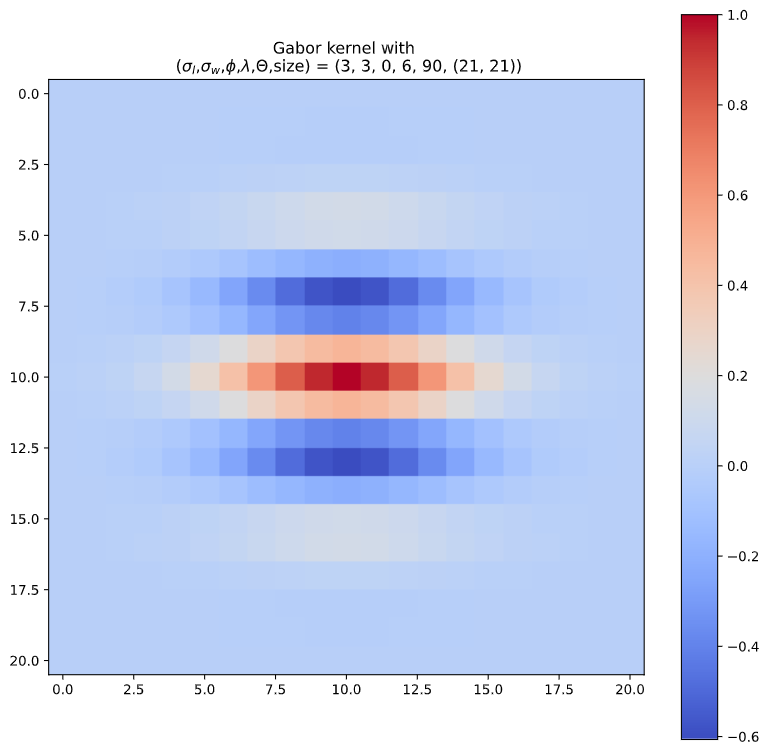
\includegraphics[width = 0.8\textwidth]{images/Gabor_90_2d.png}
    \caption{Gabor kernel with  ($\sigma_l$,$\sigma_w$,$\phi$,$\lambda$,$\theta$,size) = (3,3,0,6,90,(21,21))}
    %\label{fig:mesh1}
\end{figure}

\newpage
{\scshape EEE 482} \hfill {\scshape \large  Homework-\romannumeral2\relax} \hfill {\scshape Can Kocagil}
\smallskip
\hrule
\vspace{2mm}


\begin{figure}[ht]
    \centering
    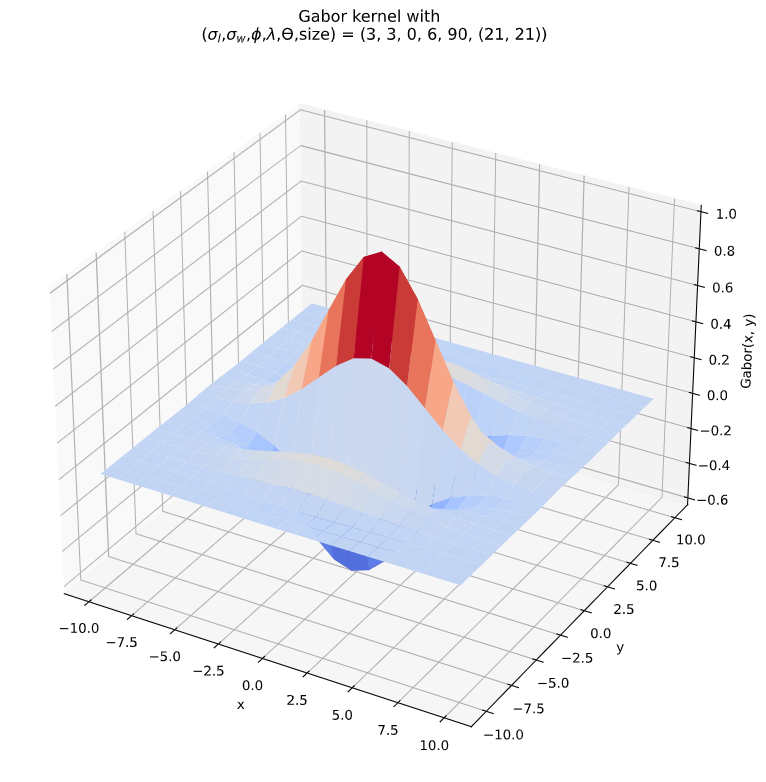
\includegraphics[width = 0.8\textwidth]{images/Gabor_90_3d.png}
    \caption{Gabor kernel with ($\sigma_l$,$\sigma_w$,$\phi$,$\lambda$,$\theta$,size) = (3,3,0,6,90,(21,21))}
    %\label{fig:mesh1}
\end{figure}

\subsection{Part E}
In this part of the question, assume that there is a separate V1 neuron with a receptive field centered on each pixel in the image with the knowledge that simple cells in V1 have Gabor receptive fields. We need to compute the responses of each neuron to the image given in hw2\_image.bmp. Finally, we are asked to discuss the function of Gabor filter. Note that this discussion is already done in previous part in detail. But, here just for the sake of simplicity, I made the similar discussion of Gabor filter. Gabor is a linear filter used for texture analysis, edge detection, feature extraction, etc. which essentially means that it analyzes whether there is any specific frequency content in the image in specific directions in a localized region around the point or region of analysis\cite{enwiki:993157632}. Frequency and orientation representations of Gabor filters are claimed by many contemporary vision scientists to be similar to those of the human visual system \cite{enwiki:993157632} as we are computing responses of each neuron to the given image . Hence, the visual cortex of some mammals can be expressed by these filters as we can see in the literature computational neuroscience. As we discuss, Gabor filter considers the optimal localization properties in both spatial \& frequency domain with orientations so that they are useful in egde detection, segmentation problems. We can consider Gabor filters as a sinusoidal oriented 2-D Gaussian filters that considers the spatial neighborhoods in cross-correlations. In a nutshell, we can think Gabor filter as linear filter such that optimal localization properties in both spatial \& frequency domain with orientations is preserved so that they become 

\newpage
{\scshape EEE 482} \hfill {\scshape \large  Homework-\romannumeral2\relax} \hfill {\scshape Can Kocagil}
\smallskip
\hrule
\vspace{2mm}

sinusoidal Gaussian envelopes. Then, let's move to computing the responses of each neuron to the image given via 2-D convolution operation as we already implemented in previous parts.


\begin{mintedbox}{python}
Gabor_result_1 = Conv2D(image[:,:,0],Gabor_90_kernel)

plt.figure(figsize=(7,7))
plt.imshow(min_max_scaler(Gabor_result_1),cmap = 'gray')
plt.title('Convolved image by DoG kernel')
plt.axis('off')
plt.show()
\end{mintedbox}


\begin{figure}[ht]
    \centering
    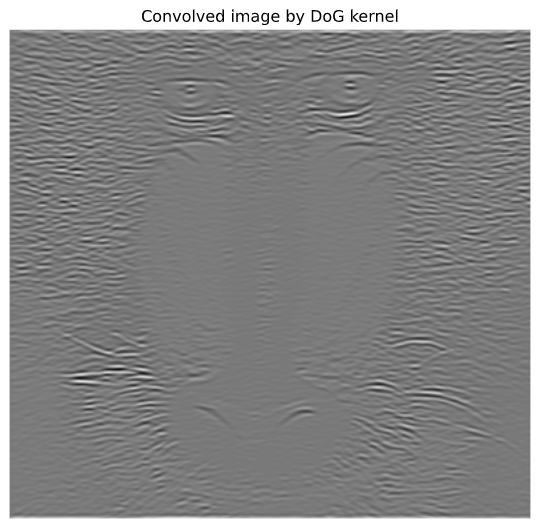
\includegraphics[width = 0.8\textwidth]{images/Gabor_conv_90.png}
    \caption{Convolved image by Gabor kernel with ($\sigma_l$,$\sigma_w$,$\phi$,$\lambda$,$\theta$,size) = (3,3,0,6,90,(21,21))}
    %\label{fig:mesh1}
\end{figure}

\newpage
{\scshape EEE 482} \hfill {\scshape \large  Homework-\romannumeral2\relax} \hfill {\scshape Can Kocagil}
\smallskip
\hrule
\vspace{2mm}

\subsection{Part F}
In this part of the question, we are asked to Construct 4 Gabors with $\theta$ = $0,\pi/2,\pi/3,\pi/2$, then compute combined neural responses to the image hw2\_image.bmp, by summing the outputs of the individual receptive fields (for different $\theta$). As we previously discuss the usage of Gabor filters and its applications in digital image domain, they are generally more than 1 Gabor filters with different orientation angles, and they are used together (by summing) to boost the performance of edge detection, texture analysis, etc as it is very common application of Gabor filter. Hence, let's construct Gabor receptive field, visualize them in both 2-D and 3-D surface then compute the individual neural responses to given image. Finally, then, we can sum the all computed neural responses to get end result. Here is the code \& visualization for For $\theta$ = $0$:

\begin{mintedbox}{python}
theta_0 = 0
Gabor_0_kernel = Gabor_Receptive_Field(theta  = theta_0, **kwargs_kernel)

plotFilter2D(Gabor_0_kernel,f'Gabor kernel with \n ($\sigma_l$,$\sigma_w$,$\phi$,$\lambda$,$\Theta$,size) = {std_l,std_w,phi,Lambda,theta_0,size}')

plotFilter3D(Gabor_0_kernel,f'Gabor kernel with \n ($\sigma_l$,$\sigma_w$,$\phi$,$\lambda$,$\Theta$,size) = {std_l,std_w,phi,Lambda,theta_0,size}',kernel_name = 'Gabor',kwargs=kwargs)

Gabor_result_2 = Conv2D(image[:,:,0],Gabor_0_kernel)
plt.figure(figsize=(7,7))
plt.imshow(min_max_scaler(Gabor_result_2),cmap = 'gray')
plt.title(f'Convolved image by DoG kernel with  \n ($\sigma_l$,$\sigma_w$,$\phi$,$\lambda$,$\Theta$,size) = {std_l,std_w,phi,Lambda,0,size}')
plt.axis('off')
plt.show()
\end{mintedbox}


\begin{figure}[ht]
    \centering
    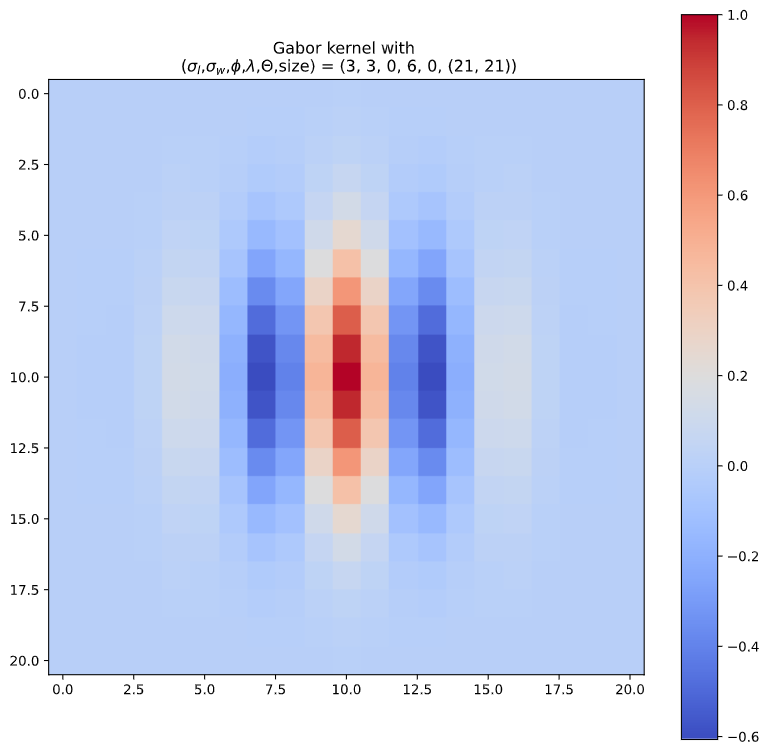
\includegraphics[width = 0.5\textwidth]{images/Gabor_0_2d.png}
    \caption{Gabor kernel with ($\sigma_l$,$\sigma_w$,$\phi$,$\lambda$,$\theta$,size) = (3,3,0,6,0,(21,21))}
    %\label{fig:mesh1}
\end{figure}



\newpage
{\scshape EEE 482} \hfill {\scshape \large  Homework-\romannumeral2\relax} \hfill {\scshape Can Kocagil}
\smallskip
\hrule
\vspace{2mm}


\begin{figure}[ht]
    \centering
    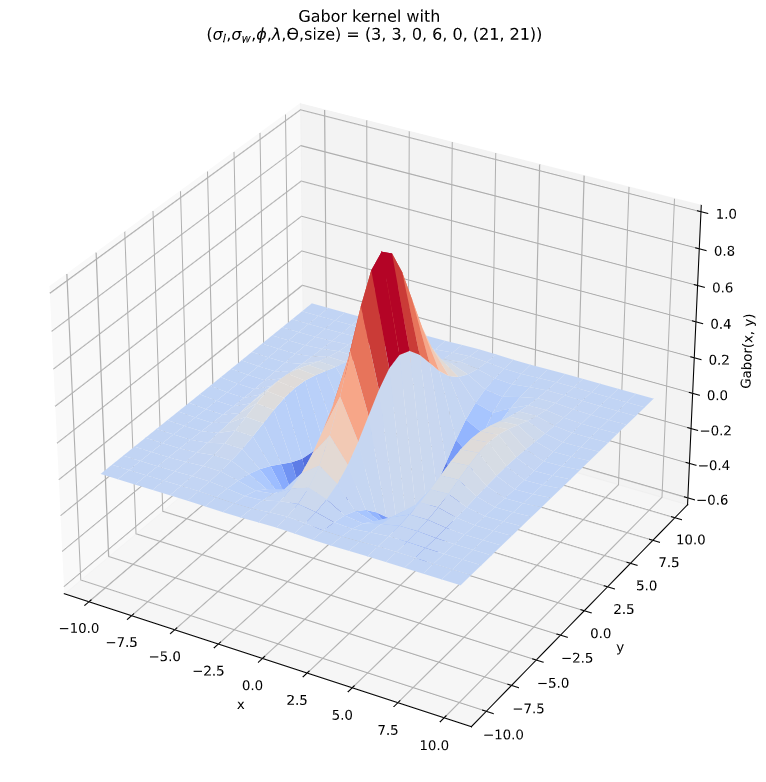
\includegraphics[width = 0.6\textwidth]{images/Gabor_0_3d.png}
    \caption{Gabor kernel with ($\sigma_l$,$\sigma_w$,$\phi$,$\lambda$,$\theta$,size) = (3,3,0,6,0,(21,21))}
    %\label{fig:mesh1}
\end{figure}





\begin{figure}[ht]
    \centering
    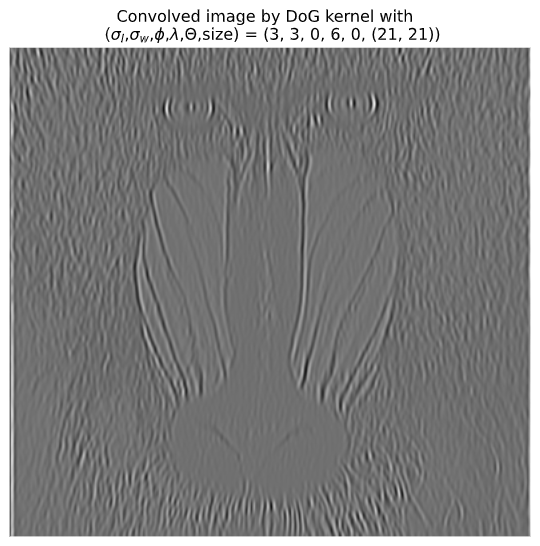
\includegraphics[width = 0.6\textwidth]{images/Gabor_conv_0.png}
    \caption{Convolved image with Gabor kernel with ($\sigma_l$,$\sigma_w$,$\phi$,$\lambda$,$\theta$,size) = (3,3,0,6,0,(21,21))}
    %\label{fig:mesh1}
\end{figure}



\newpage
{\scshape EEE 482} \hfill {\scshape \large  Homework-\romannumeral2\relax} \hfill {\scshape Can Kocagil}
\smallskip
\hrule
\vspace{2mm}

Here is the code \& visualization for $\theta$ = $\pi/6$.
\begin{mintedbox}{python}
theta_30 = np.pi / 6

Gabor_30_kernel = Gabor_Receptive_Field(theta = theta_30,**kwargs_kernel)
plotFilter2D(Gabor_30_kernel,f'Gabor kernel with \n ($\sigma_l$,$\sigma_w$,$\phi$,$\lambda$,$\Theta$,size) = {std_l,std_w,phi,Lambda,30,size}')

plotFilter3D(Gabor_30_kernel,f'Gabor kernel with \n ($\sigma_l$,$\sigma_w$,$\phi$,$\lambda$,$\Theta$,size) = {std_l,std_w,phi,Lambda,30,size}',kernel_name = 'Gabor',kwargs=kwargs)


Gabor_result_3 = Conv2D(image[:,:,0],Gabor_30_kernel)


plt.figure(figsize=(7,7))
plt.imshow(min_max_scaler(Gabor_result_3),cmap = 'gray')
plt.title(f'Convolved image by DoG kernel with  \n ($\sigma_l$,$\sigma_w$,$\phi$,$\lambda$,$\Theta$,size) = {std_l,std_w,phi,Lambda,30,size}')
plt.axis('off')
plt.show()
\end{mintedbox}

\begin{figure}[ht]
    \centering
    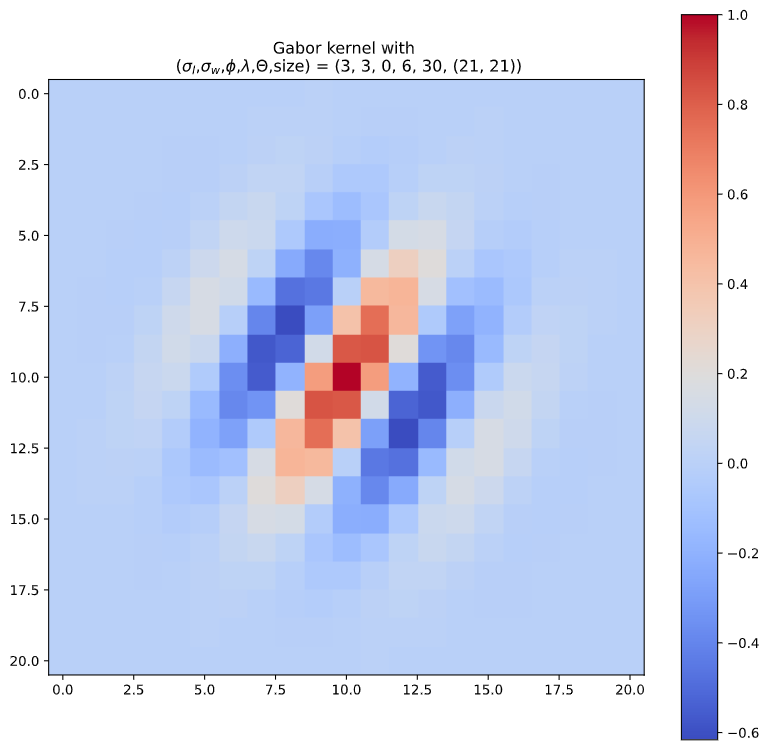
\includegraphics[width = 0.6\textwidth]{images/Gabor_30_2d.png}
    \caption{Gabor kernel with ($\sigma_l$,$\sigma_w$,$\phi$,$\lambda$,$\theta$,size) = (3,3,0,6,30,(21,21))}
    %\label{fig:mesh1}
\end{figure}

\newpage
{\scshape EEE 482} \hfill {\scshape \large  Homework-\romannumeral2\relax} \hfill {\scshape Can Kocagil}
\smallskip
\hrule
\vspace{2mm}

\begin{figure}[ht]
    \centering
    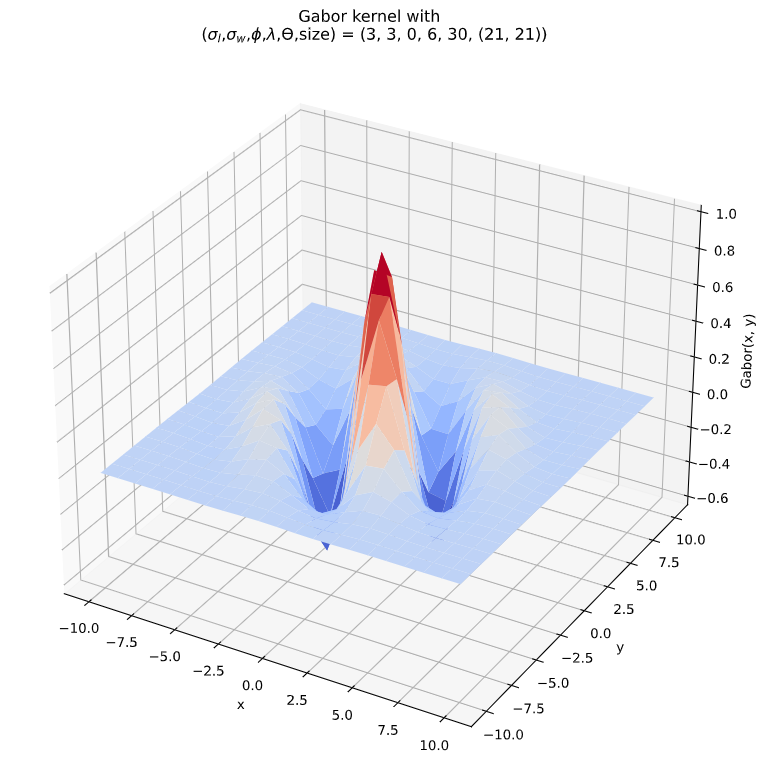
\includegraphics[width = 0.6\textwidth]{images/Gabor_30_3d.png}
    \caption{Gabor kernel with ($\sigma_l$,$\sigma_w$,$\phi$,$\lambda$,$\theta$,size) = (3,3,0,6,30,(21,21))}
    %\label{fig:mesh1}
\end{figure}


\begin{figure}[ht]
    \centering
    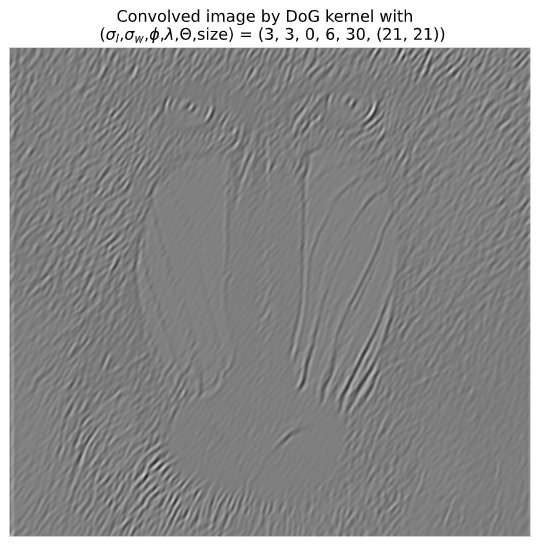
\includegraphics[width = 0.6\textwidth]{images/Gabor_conv_30.png}
    \caption{Convolved image with Gabor kernel with ($\sigma_l$,$\sigma_w$,$\phi$,$\lambda$,$\theta$,size) = (3,3,0,6,30,(21,21))}
    %\label{fig:mesh1}
\end{figure}



\newpage
{\scshape EEE 482} \hfill {\scshape \large  Homework-\romannumeral2\relax} \hfill {\scshape Can Kocagil}
\smallskip
\hrule
\vspace{2mm}

Here is the code \& visualization for $\theta$ = $\pi/3$.
\begin{mintedbox}{python}
theta_60 = np.pi / 3

Gabor_60_kernel = Gabor_Receptive_Field(theta = theta_60,**kwargs_kernel)

plotFilter2D(Gabor_60_kernel,
title = f'Gabor kernel with \n ($\sigma_l$,$\sigma_w$,$\phi$,$\lambda$,$\theta$,size) = {std_l,std_w,phi,Lambda,60,size}'

)

plotFilter3D(Gabor_60_kernel,f'Gabor kernel with \n ($\sigma_l$,$\sigma_w$,$\phi$,$\lambda$,$\theta$,size) = {std_l,std_w,phi,Lambda,60,size}',kernel_name = 'Gabor',kwargs=kwargs)



Gabor_result_4 = Conv2D(image[:,:,0],Gabor_60_kernel)


plt.figure(figsize=(7,7))
plt.imshow(min_max_scaler(Gabor_result_4),cmap = 'gray')
plt.title(f'Convolved image by DoG kernel with  \n ($\sigma_l$,$\sigma_w$,$\phi$,$\lambda$,$\theta$,size) = {std_l,std_w,phi,Lambda,60,size}')
plt.axis('off')
plt.show()


\end{mintedbox}

\begin{figure}[ht]
    \centering
    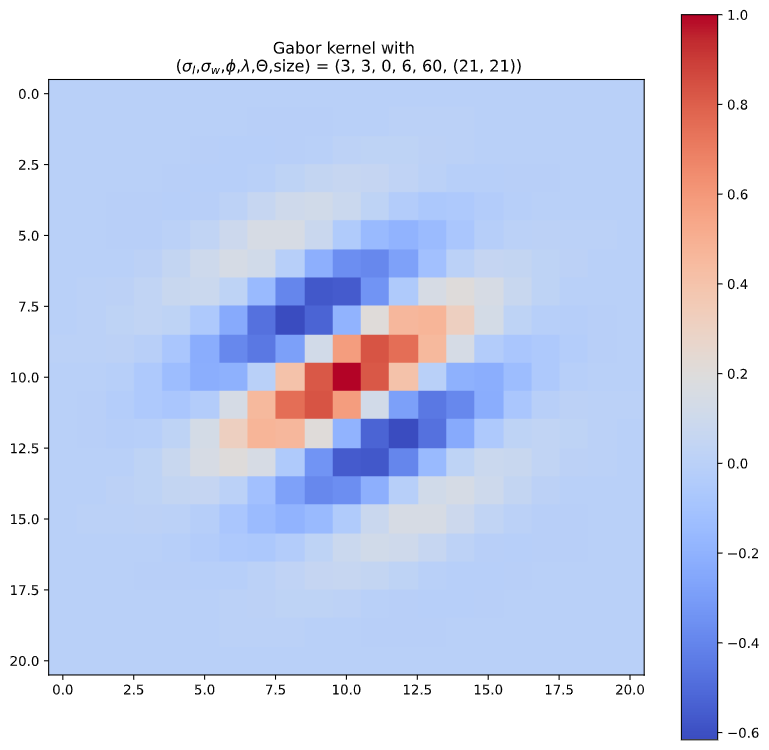
\includegraphics[width = 0.6\textwidth]{images/Gabor_60_2d.png}
    \caption{Gabor kernel with ($\sigma_l$,$\sigma_w$,$\phi$,$\lambda$,$\theta$,size) = (3,3,0,6,60,(21,21))}
    %\label{fig:mesh1}
\end{figure}

\newpage
{\scshape EEE 482} \hfill {\scshape \large  Homework-\romannumeral2\relax} \hfill {\scshape Can Kocagil}
\smallskip
\hrule
\vspace{2mm}

\begin{figure}[ht]
    \centering
    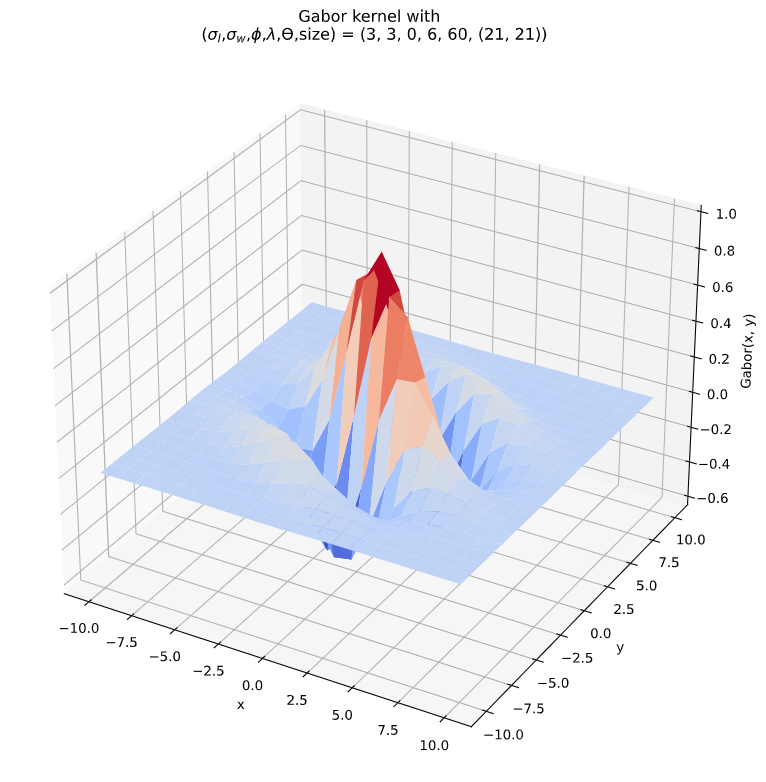
\includegraphics[width = 0.6\textwidth]{images/Gabor_60_3d.png}
    \caption{Gabor kernel with ($\sigma_l$,$\sigma_w$,$\phi$,$\lambda$,$\theta$,size) = (3,3,0,6,60,(21,21))}
    %\label{fig:mesh1}
\end{figure}


\begin{figure}[ht]
    \centering
    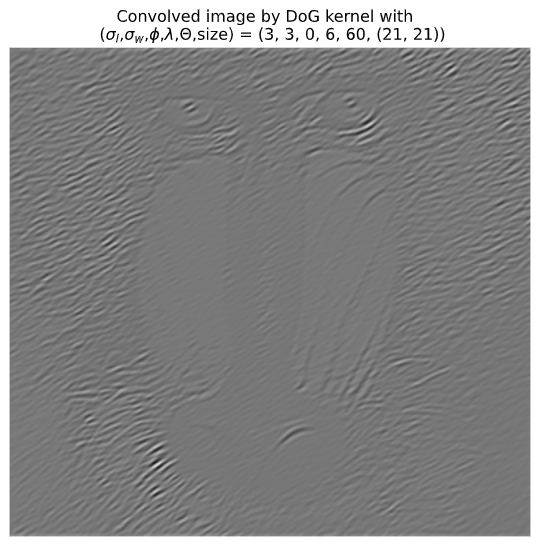
\includegraphics[width = 0.6\textwidth]{images/Gabor_conv_60.png}
    \caption{Convolved image with Gabor kernel with ($\sigma_l$,$\sigma_w$,$\phi$,$\lambda$,$\theta$,size) = (3,3,0,6,60,(21,21))}
    %\label{fig:mesh1}
\end{figure}




\newpage
{\scshape EEE 482} \hfill {\scshape \large  Homework-\romannumeral2\relax} \hfill {\scshape Can Kocagil}
\smallskip
\hrule
\vspace{2mm}

Let's combine the results we obtained in previous pages, to do that we need sum images after applying Gabor kernel with different orientations with $\theta$ = $\pi/2$,$\pi/3$,$\pi/6$,$0$. Let's see the code for combining, plotting and edge detection operation.


\begin{mintedbox}{python}
composite_gabor = Gabor_result_1 + Gabor_result_2 + Gabor_result_3 + Gabor_result_4
img = np.array(min_max_scaler(composite_gabor) * 255, dtype = np.uint8)

plt.figure(figsize=(7,7))
plt.imshow(composite_gabor,cmap = 'gray')
plt.title('Output of combined Gabol kernels')
plt.axis('off')
plt.show()

plt.figure(figsize=(7,7))
plt.imshow(manuel_thresholding(img,127),cmap = 'gray')
plt.title('Thresholded image of output of combined Gabol kernels')
plt.axis('off')
plt.show()
\end{mintedbox}

\begin{figure}[ht]
    \centering
    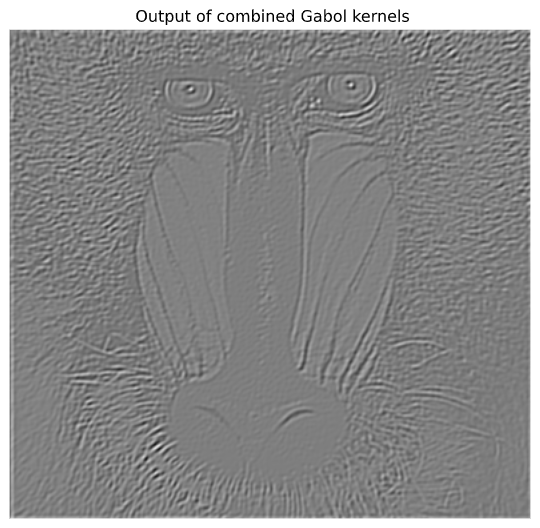
\includegraphics[width = 0.6\textwidth]{images/comb_conv.png}
    \caption{Output of combined results of Gabor responses}
    %\label{fig:mesh1}
\end{figure}

\newpage
{\scshape EEE 482} \hfill {\scshape \large  Homework-\romannumeral2\relax} \hfill {\scshape Can Kocagil}
\smallskip
\hrule
\vspace{2mm}

\begin{figure}[ht]
    \centering
    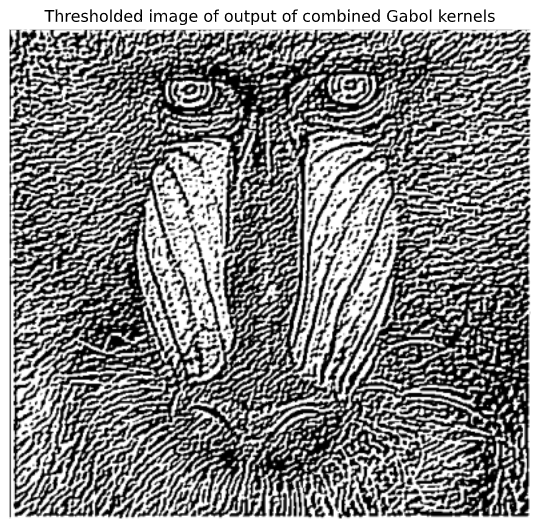
\includegraphics[width = 0.6\textwidth]{images/comb_conv_thres.png}
    \caption{Thresholded image obtained by the output of combined results of Gabor responses}
    %\label{fig:mesh1}
\end{figure}

Let's also make a grid of figure that consist of image obtained by the output of combined results of Gabor responses and DoG kernel, just for sake of the simplicity for comparison.


\begin{figure}[ht]
    \centering
    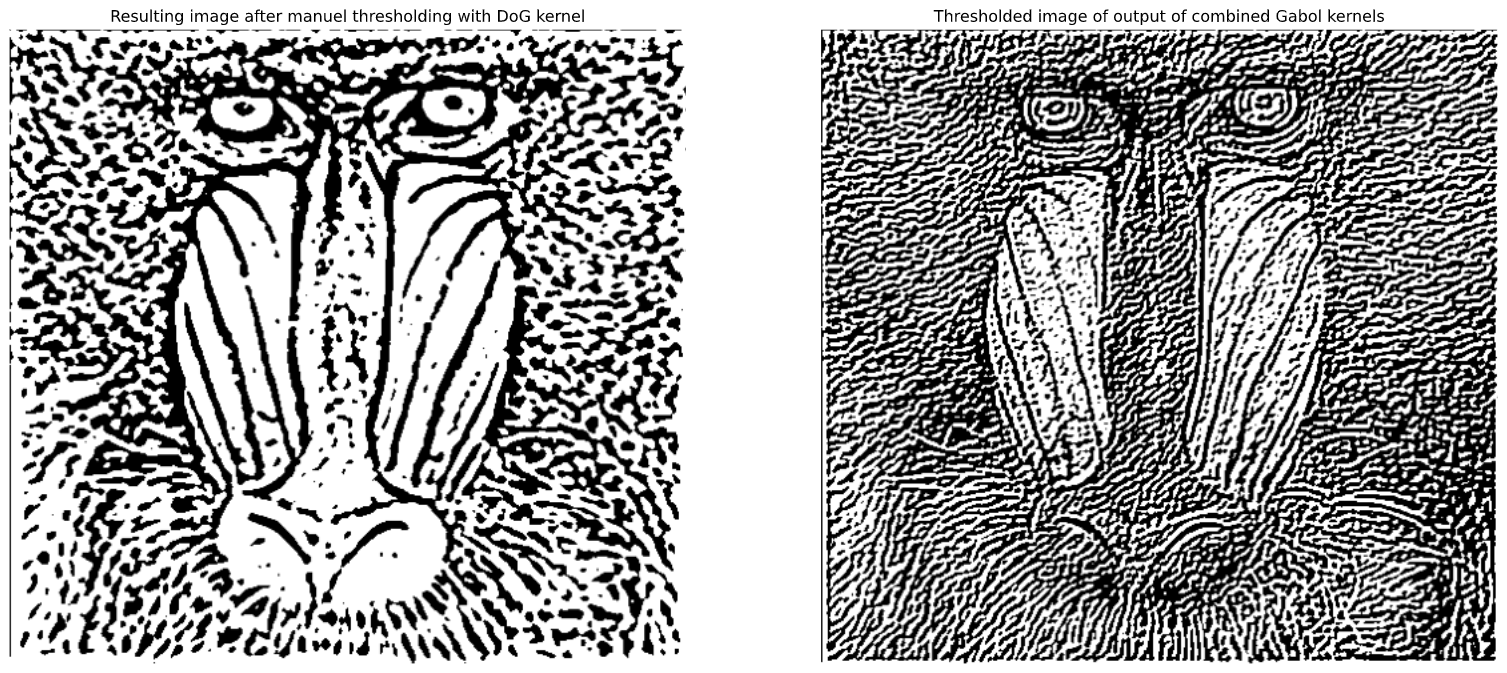
\includegraphics[width = 1\textwidth]{images/last.png}
    \caption{Comparison figure between image obtained by the output of combined results of Gabor responses and DoG kernel}
    %\label{fig:mesh1}
\end{figure}

\newpage
{\scshape EEE 482} \hfill {\scshape \large  Homework-\romannumeral2\relax} \hfill {\scshape Can Kocagil}
\smallskip
\hrule
\vspace{2mm}

As we can see clearly from the grid figure from above, the combination of Gabor filters responses performed much more better than single DoG kernel from the edge detection \& feature extraction performance. There are various reasons for that such as Gabor filters considers the orientation and also we combine 4 different orientations. The extracted features, in our case, mostly edges, from the Gabor filters are spatially better than the ones extracted from the DoG kernel since we can see the neighbourhood relations much more clearly. As a further improvements onto Gabor filters, the rule of thumb approach in real image processing application is the usage of bank of Gabor filters as we did in this part. So, we can add much more orientations then construct a bank of Gabor filters to improve the features quality. Also, as we saw, there are parameters of Gabor filters such as $\pi$,$\sigma$,$\lambda$, etc., that can be further tuned to make improvements. Specifically, we can tune the $\lambda$ to change the wavelength of the sinusoidal components, $\theta$ to get different orientations of the normal to the parallel stripes of Gabor kernel. Also, we have a phase effect $\phi$ so that we can give more/less offset to sinusoidal function to get better results. As a Gaussian part of the Gabor, we can also tune the $\sigma$ parameters to arrange the envelope of the Gaussian. Furthermore, some Gabor filters uses additional $\varphi$ parameter to adjust the spatial aspect ratio and ellipticity of the support of the Gabor kernel, i.e., new 2-D Gabor function becomes with the new parameter $\varphi$ as follows


\begin{equation}
    D(\vec{x}^{\,}) = \exp{\left( - (\vec{k}^{\,}(\theta) \cdot \vec{x}^{\,})^2 / 2\sigma_l^2 - (\vec{k_\bot}^{\,}(\theta) \cdot \varphi\vec{x}^{\,})^2 / 2\sigma_w^2 \right)} \cos{\left(2\pi \frac{\vec{k_\bot}^{\,}(\theta) \cdot \vec{x}^{\,}}{\lambda} + \phi \right)}
\end{equation}


Briefly, let's sum it up in one paragraph. Increasing the wavelenth $\theta$ produces a thicker stripes that can be effective in some situations such that the extracted features quality increases. We can create different orientations of Gabor function, we can tune the $\varphi$ to control over the aspect ratio so that it fits into specific situation then we can also tune the bandwith of the Gabor function $\sigma$ to arrange the envelope of the Gaussian component of Gabor and much more. Finally, experimenting with the parameters of the Gabor kernel and its application with the bank of Gabor filters will eventually extract spatially meaningful informations from the natural images that can have random Gaussian noise in real life situations.




\newpage
{\scshape EEE 482} \hfill {\scshape \large  Homework-\romannumeral2\relax} \hfill {\scshape Can Kocagil}
\smallskip
\hrule
\vspace{2mm}



\section{Source Code}


\begin{mintedbox}{python}
# -*- coding: utf-8 -*-
"""EEE482_Can_Kocagil_21602218_Hw_2.ipynb

Automatically generated by Colaboratory.

Original file is located at
    https://colab.research.google.com/drive/14TTuu1Vul3FC5lRg3JCOQHyy4D4JDL50
"""

import numpy as np 
import scipy.io as io
import matplotlib.pyplot as plt

#pwd

#ls

data = io.loadmat('c2p3.mat')
print(data.keys())

counts = data['counts']
stim = data['stim']

print(f"The shape of the counts data {counts.shape}")
print(f"The shape of the Stimilus data {stim.shape}")

def STA(stim:np.ndarray,rho:np.ndarray,num_timesteps:int) -> np.ndarray:
    """
        Given the stimilus, rho (spike train) and number of time steps, computes 
        Spike-Triggered-Average (STA). The spike-triggered average (STA) is a measure to relate a                     continuous signal and a simultaneously recorded spike train. It represents the average  signal  taken         at the times of spike occurrences and with proper normalization is equivalent to the   cross-correlation between the continuous signal and the spike  -train. The STA provides an estimate of a neuron's linear receptive field.


            Arguments:
                - stim (np.ndarray)   : Stimulus data to be subjected
                - rho  (np.ndarray)   : Time-series Spike-train data 
                - num_timesteps (int) : Number of timesteps before spike

            Returns:
                - _STA (np.ndarray)    : Averaged Stimulis data taken at spike occurrences



    """

    # Creating zero matrix for STA:
    stim_h,stim_w = stim.shape[:2]
    _STA = np.zeros((stim_h,stim_w,num_timesteps))

    # Finding spike times + num_timesteps
    spike_times = rho[num_timesteps:].nonzero()[0] + num_timesteps


    print(f'There are {len(spike_times)} of spikes.')

    for idx_spike in spike_times:
        _STA += stim[:,:,idx_spike - num_timesteps:idx_spike]

    _STA = _STA.astype(np.float)
    _STA /= len(spike_times)

    return _STA

num_timesteps = 10
sta = STA(stim,counts,num_timesteps)

kwargs = dict(
    cmap = 'gray',
    vmin = sta.min(),
    vmax = sta.max()      
)


for i in np.arange(num_timesteps):
    plt.figure()
    plt.imshow(sta[:,:,i],**kwargs)
    plt.title(f"{num_timesteps - i} steps before the spike")
    plt.axis('off')
    plt.savefig(f"{num_timesteps - i}.png")

fig,axs = plt.subplots(1,2,figsize = (20,40)) 
axs[0].imshow(np.sum(sta,axis = 0),**kwargs)
axs[0].set_title(f"Row sum of STA")
axs[1].imshow(np.sum(sta,axis = 1),**kwargs)
axs[1].set_title(f"Column sum of STA")


plt.show()
plt.savefig('SpatialDimensionSummationofSTANew' + '.png')

project_stim = np.array([np.sum(sta[:,:, num_timesteps - 1] * _stim) for _stim in np.swapaxes(stim,0,2)]) 
project_stim /= project_stim.max()
kwargs = dict(
    bins=100, 
    alpha=.8,
    rwidth=.66,
   
)
plt.figure(figsize=(10, 5))
plt.hist(project_stim,color='g', **kwargs)
plt.title('Histogram of Stimilus Projections on STA')
plt.ylabel('Spike Frequency')
plt.xlabel('Normalized Stimulus Projection')
plt.show()
plt.savefig('HistogramSTA.png')

spike_times = counts.nonzero()[0]

project_stim_nonzero = np.array([np.sum(sta[:,:, num_timesteps - 1] * stim[:,:,i]) for i in spike_times]) 
project_stim_nonzero /= project_stim_nonzero.max()


plt.figure(figsize=(10, 5))
plt.hist(project_stim_nonzero, **kwargs,color='orange')
plt.title('Histogram of Stimilus Projections on STA for non-zero spikes')
plt.ylabel('Spike Frequency')
plt.xlabel('Normalized Stimulus Projection')
plt.show()

plt.figure(figsize=(10, 5))
plt.hist(project_stim, **kwargs)
plt.title('Comparison Histogram of Stimilus Projections on STA')
plt.hist(project_stim_nonzero, **kwargs)
plt.ylabel('Spike Frequency')
plt.xlabel('Normalized Stimulus Projection')
plt.legend(['For all Spikes','For nonzero spikes'])
plt.show()

def DoG_Receptive_Field(std_c:int,std_s:int,size:int) -> np.ndarray:
    """
        Construct an on-center difference-of-gaussians (DoG) center-surround receptive field
        centered at 0 with the given size. Generally, the Difference of Gaussian module is a             filter that  identifies edges.Additionally, DoG is a feature enhancement algorithm that          involves the subtraction of one Gaussian blurred version of an original image from               another, less blurred version of the original


            Arguments:
                - std_c (int) : Standard deviation of lower sigma
                - std_s (int) : Standard deviation of higher sigma
                - size  (int) : Size of DoG kernel

            Returns:
               - DoG_kernel (np.ndarray) : DoG kernel with given (size,size)

    """


    import math

    # Computing lower sigma kernel:
    low_sigma_kernel  = np.fromfunction(
        lambda x, y: (1/(2*math.pi*std_c**2)) * math.e ** ((-1*((x-(size-1)/2)** 2+(y-(size-1)/2)**2))/(2*std_c**2)), (size, size)        
        )

    # Computing higher sigma kernel:
    high_sigma_kernel = np.fromfunction(
        lambda x, y: (1/(2*math.pi*std_s**2)) * math.e ** ((-1*((x-(size-1)/2)**2+(y-(size-1)/2)**2))/(2*std_s**2)), (size, size)
        )

    # DoG kernel:
    DoG_kernel = low_sigma_kernel - high_sigma_kernel


    return DoG_kernel

DoG_kernel = DoG_Receptive_Field(**
dict(
    size = 21,
    std_c = 2,
    std_s = 4

))

def plotFilter2D(kernel:np.ndarray,title:str,
                 cmap:str='coolwarm',
                 figsize:tuple = (10,10),
                 kwargs:dict = None) -> None:

    """
        Given the kernel, plot the kernel in 2-D surface.

            Arguments:
                - kernel (np.ndarray) : Kernel to be plotted
                - title  (str)        : Title of the figure
                - cmap   (str)        : Texture of the figure
                - figsize (tuple)     : Figure size
                - kwargs (dict)       : Additional orguments to plot if exists

            Returns:
                - None



    """

    plt.figure(figsize = figsize)

    if kwargs is not None:
        plt.imshow(kernel,cmap=cmap,**kwargs)
    else:
        plt.imshow(kernel,cmap=cmap)       
    
    plt.title(title)
    plt.colorbar()
    plt.show()




def plotFilter3D(kernel:np.ndarray,title:str,
                 kernel_name:str, 
                 cmap:str='coolwarm',
                 figsize:tuple = (10,10),
                 kwargs:dict = None) -> None:

    """
        Given the kernel, plot the kernel in 2-D surface.

            Arguments:
                - kernel (np.ndarray) : Kernel to be plotted
                - title  (str)        : Title of the figure
                - kernel_name (str)   : The name of the filter/kernel
                - cmap   (str)        : Texture of the figure
                - figsize (tuple)     : Figure size
                - kwargs (dict)       : Additional orguments to plot if exists

            Returns:
                - None



    """

    fig_3D = plt.figure(figsize = (10,10))
    size = kernel.shape[0]
    ax_3D = plt.axes(projection='3d')
    x,y = np.meshgrid(
        np.arange( - int(size / 2), 1 + int(size / 2)),
        np.arange( - int(size / 2), 1 + int(size / 2))
                )
    
    
    if kwargs is not None:
        ax_3D.plot_surface(x, y, kernel,cmap = cmap, **kwargs)
    else:
        ax_3D.plot_surface(x, y,kernel, cmap = cmap)   
    
    ax_3D.set_xlabel('x')
    ax_3D.set_ylabel('y')
    ax_3D.set_zlabel(f'{kernel_name}(x, y)')
    plt.title(title)
    plt.show()

kwargs = dict(
    rstride=1,
    cstride=1,     
    edgecolor='none'
)


plotFilter2D(DoG_kernel,f'Difference of Gaussian (DoG) kernel with Stds {(2,4)} in 21x21 form')

plotFilter3D(DoG_kernel,f'Difference of Gaussian (DoG) kernel with Stds {(2,4)} in 21x21 form','DoG', kwargs = kwargs)

image = plt.imread('hw2_image.bmp')
plt.figure(figsize=(10,10))
plt.imshow(image)
plt.axis('off')
plt.show()

class _Window(object):
  """
    This class creates a generator that slide over the given image with
    predefined step and window size.

      Attributes:
        - image      : input image to be sliding
        - step_size  : it determines how much slice the generator extract
        - dims       : resulting image's dimensions

      Methods:
        - __iter__   : creates a generator over the image with given patch dimensions

  """
  def __init__(self,image : np.ndarray, step_size:tuple, dims: tuple):
    """ 
      Creates an constructor for _Window class, this method encapsulates
      all necessary data to generate windows over image.  

    """
    self.image = image 
    self.dims = dims 
    self.step_size = step_size

  def __iter__(self):
    """ Generator function to window over image. """
    for x in range(self.dims[0]):
      for y in range(self.dims[1]):
        yield self.image[x:x + self.step_size[0], y:y + self.step_size[1]]


def Conv2D(source_image : np.ndarray, kernel: np.ndarray) -> np.ndarray:
  """
   Convolution is the process of adding each element of the image to its local neighbors,           weighted by the kernel. This is related to a form of mathematical convolution.
   
      Arguments:
        - source_image   (np.ndarray) : Gray scale image to be convolved
        - kernel         (np.ndarray) : Kernel to be sliding over the image

      Returns:
        - conv_image     (np.ndarray) : Resulting convolved image
  """

  assert (len(source_image.shape)   == 2), "Image is not gray scale" 
  assert (len(kernel.shape) == 2), "Kernel is not in required size"      
  
  source_image =  np.asarray(source_image).clip(0,255).copy()
  H,W = source_image.shape
  k_h,k_w = kernel.shape
  padded_image = np.pad(array = source_image, pad_width = max(k_w,k_w) // 2 + 1, mode = 'constant')

  new_H,new_W = padded_image.shape
  h_pad , w_pad  =  (new_H - H) , (new_W - W)

  # Creating sliding window:
  image_window = _Window(padded_image,(k_h,k_w),(new_H - h_pad, new_W - w_pad))

  #kernel = np.flipud(np.fliplr(kernel))
  # Main operation:
  conv_image = [(patch * kernel).sum() for patch in image_window]
  
  return np.array(conv_image).reshape(H,W)



def min_max_scaler(matrix : np.ndarray)-> np.ndarray :
  """
    Given the matrix, apply normalization as follow:

        norm_matrix = (matrix - min_val) / (max_val - min_val)

    Arguments:
      -  matrix     (np.ndarray) : Input Matrix

    Returns:
      - norm_matrix (np.ndarray) : Normalized version of matr

  """
  matrix = np.asarray(matrix).copy()
  max_val = matrix.max()
  min_val = matrix.min()

  return (matrix - min_val) / (max_val - min_val)

if (image[:,:,0] == image[:,:,1]).all() and \
   (image[:,:,0] == image[:,:,2]).all() and \
   (image[:,:,1] == image[:,:,2]).all():

   print('True')


gray_image = image[:,:,0]
filtered_image = Conv2D(gray_image,DoG_kernel)

plt.figure(figsize=(7,7))
plt.imshow(min_max_scaler(filtered_image),cmap = 'gray')
plt.title('Convolved image by DoG kernel')
plt.axis('off')
plt.show()

def otsu_threshold(source_image: np.ndarray) -> np.ndarray:
    """
    Otsu's automatic thresholding method that seperates background and
    foreground of image with automatically computed threshold value. This 
    threshold is computed via minimizing the within-class varicance or 
    maximing the inter-class variability that yields same results. However,
    note that computed threshold value by maximizing the inter-class variance
    is more computationally efficient method. 

      Arguments:
        - source_image (np.ndarray) : Source image to be thresholded by Otsu

      Returns:
        - thres_image  (np.ndarray) : Resulting image after applying Otsu's method
 

  """

    assert (len(source_image.shape) == 2), "Image is not gray scale"     
    
    source_image =  np.asarray(source_image).clip(0,255).copy()

    hist =  [np.sum(pixel == source_image) for pixel in np.arange(256)]

    
    otsu_thres = 0
    var = 0
    max_val = 256
    
    for thres in np.arange(256):

      # For first class, mean and variance:
      w_0 = sum(pixel for pixel in hist[:thres])
      mu_0 = sum([i * hist[i] for i in range(thres)]) / w_0 if w_0 > 0 else 0   

      # For second class, mean and variance:
      w_1 = sum(pixel for pixel in hist[thres:])          
      mu_1 = sum([j * hist[j] for j in range(thres, max_val)]) / w_1 if w_1 > 0 else 0

      # calculating inter-class variance         
      s = w_0 * w_1 * (mu_0 - mu_1) ** 2

      # Set threshold if new inter class variance is bigger than previous
      otsu_thres = thres - 1 if s > var else otsu_thres
      var = s if s > var else var

    print(f'Self written Otsu threshold value is {otsu_thres}')  

    # Apply thresholding: Hence
    source_image[source_image >= otsu_thres] = 255
    source_image[source_image < otsu_thres] = 0

    return source_image.astype(np.uint8)

def manuel_thresholding(source_image: np.ndarray,threshold:int) -> np.ndarray:
    """
        Given the source image and threshold, apply thresholding (i.e., setting all values
        above a certain threshold to 1 and the remainder to 0.

            Arguments:
                - source_image (np.ndarray) : Source image to be thresholded
                - threshold    (int)        : Threshold value

            Returns:   
                - thres_image  (np.ndarray) : Resulting image after applying threshold



    """

    
    assert (len(source_image.shape) == 2), "Image is not gray scale"     
    
    source_image =  np.asarray(source_image).clip(0,255).copy()



    # Apply thresholding:
    source_image[source_image >= threshold] = 255
    source_image[source_image < threshold] = 0

    return source_image.astype(np.uint8)

img = np.array(min_max_scaler(filtered_image) * 255, dtype = np.uint8)


plt.figure(figsize=(7,7))
plt.imshow(manuel_thresholding(img,115),cmap = 'gray')
plt.title('Resulting image after manuel thresholding')
plt.axis('off')
plt.show()


img = np.array(min_max_scaler(filtered_image) * 255, dtype = np.uint8)
plt.figure(figsize=(7,7))
import cv2
plt.imshow(cv2.threshold(img,0,255,cv2.THRESH_BINARY+cv2.THRESH_OTSU)[1],cmap = 'gray')
plt.title('Resulting image after otsu thresholding')
plt.axis('off')
plt.show()



img = np.array(min_max_scaler(filtered_image) * 255, dtype = np.uint8)
plt.figure(figsize=(7,7))
plt.imshow(otsu_threshold(img),cmap = 'gray')
plt.title('Convolved image by DoG kernel')
plt.axis('off')
plt.show()

def Gabor_Receptive_Field(std_l:int,std_w:int,
                          theta:float,Lambda:int,
                          psi:int, size:tuple) -> np.ndarray:
    """
        Gabor Receptive Field is a linear filter used for texture analysis, which essentially             means that it analyzes whether there is any specific frequency content in the image in            specific directions in a localized region around the point or region of analysis


            Arguments:
                - std_l  (int)   : Standard deviation of lower sigma
                - std_w  (int)   : Standard deviation of higher sigma                
                - theta  (float) : Orientation
                - Lambda (int)   : Gabor filter parameter 
                - psi    (int)   : Gabor filter parameter
                - size   (tuple) : Size of Gabor kernel

            Returns:
               - Gabor_kernel (np.ndarray) : Gabor kernel with given (size,size)

    """


    import math

    x, y = np.meshgrid(np.arange(- int(size[0] / 2), 1 + int(size[0] / 2)),
                       np.arange(- int(size[1] / 2), 1 + int(size[1] / 2)))


    # Rotation
    x_theta = x * np.cos(theta) + y * np.sin(theta)
    y_theta = -x * np.sin(theta) + y * np.cos(theta)

    # Main function for creating Gabor filter:
    Gabor_kernel = np.exp(-.5 * (x_theta ** 2 / std_l ** 2 + y_theta ** 2 / std_w ** 2)) * np.cos(2 * np.pi / Lambda * x_theta + psi)


    return Gabor_kernel

theta_90 = np.pi / 2
size = (21,21)
kwargs_kernel = dict(
        std_l = 3,
        std_w = 3,
        psi = 0,
        Lambda = 6,
        size = size
)

std_l = 3
std_w = 3
phi = 0
Lambda = 6
size = size

Gabor_90_kernel = Gabor_Receptive_Field(theta = theta_90,**kwargs_kernel)


kwargs = dict(
    rstride=1,
    cstride=1,     
    edgecolor='none'

)

plotFilter2D(Gabor_90_kernel,f'Gabor kernel with \n ($\sigma_l$,$\sigma_w$,$\phi$,$\lambda$,$\Theta$,size) = {std_l,std_w,phi,Lambda,90,size}'
)



plotFilter3D(Gabor_90_kernel,f'Gabor kernel with \n ($\sigma_l$,$\sigma_w$,$\phi$,$\lambda$,$\Theta$,size) = {std_l,std_w,phi,Lambda,90,size}',kernel_name = 'Gabor',kwargs=kwargs)


Gabor_result_1 = Conv2D(image[:,:,0],Gabor_90_kernel)

plt.figure(figsize=(7,7))
plt.imshow(min_max_scaler(Gabor_result_1),cmap = 'gray')
plt.title('Convolved image by DoG kernel')
plt.axis('off')
plt.show()

theta_0 = 0
Gabor_0_kernel = Gabor_Receptive_Field(theta  = theta_0, **kwargs_kernel)

plotFilter2D(Gabor_0_kernel,f'Gabor kernel with \n ($\sigma_l$,$\sigma_w$,$\phi$,$\lambda$,$\Theta$,size) = {std_l,std_w,phi,Lambda,theta_0,size}')

plotFilter3D(Gabor_0_kernel,f'Gabor kernel with \n ($\sigma_l$,$\sigma_w$,$\phi$,$\lambda$,$\Theta$,size) = {std_l,std_w,phi,Lambda,theta_0,size}',kernel_name = 'Gabor',kwargs=kwargs)


Gabor_result_2 = Conv2D(image[:,:,0],Gabor_0_kernel)


plt.figure(figsize=(7,7))
plt.imshow(min_max_scaler(Gabor_result_2),cmap = 'gray')
plt.title(f'Convolved image by DoG kernel with  \n ($\sigma_l$,$\sigma_w$,$\phi$,$\lambda$,$\Theta$,size) = {std_l,std_w,phi,Lambda,0,size}')
plt.axis('off')
plt.show()

theta_30 = np.pi / 6

Gabor_30_kernel = Gabor_Receptive_Field(theta = theta_30,**kwargs_kernel)
plotFilter2D(Gabor_30_kernel,f'Gabor kernel with \n ($\sigma_l$,$\sigma_w$,$\phi$,$\lambda$,$\Theta$,size) = {std_l,std_w,phi,Lambda,30,size}')

plotFilter3D(Gabor_30_kernel,f'Gabor kernel with \n ($\sigma_l$,$\sigma_w$,$\phi$,$\lambda$,$\Theta$,size) = {std_l,std_w,phi,Lambda,30,size}',kernel_name = 'Gabor',kwargs=kwargs)


Gabor_result_3 = Conv2D(image[:,:,0],Gabor_30_kernel)


plt.figure(figsize=(7,7))
plt.imshow(min_max_scaler(Gabor_result_3),cmap = 'gray')
plt.title(f'Convolved image by DoG kernel with  ($\sigma_l$,$\sigma_w$,$\phi$,$\lambda$,$\Theta$,size) = {std_l,std_w,phi,Lambda,30,size}')
plt.axis('off')
plt.show()

theta_60 = np.pi / 3

Gabor_60_kernel = Gabor_Receptive_Field(theta = theta_60,**kwargs_kernel)

plotFilter2D(Gabor_60_kernel,
title = f'Gabor kernel with  ($\sigma_l$,$\sigma_w$,$\phi$,$\lambda$,$\Theta$,size) = {std_l,std_w,phi,Lambda,60,size}'

)

plotFilter3D(Gabor_60_kernel,f'Gabor kernel with ($\sigma_l$,$\sigma_w$,$\phi$,$\lambda$,$\Theta$,size) = {std_l,std_w,phi,Lambda,60,size}',kernel_name = 'Gabor',kwargs=kwargs)



Gabor_result_4 = Conv2D(image[:,:,0],Gabor_60_kernel)


plt.figure(figsize=(7,7))
plt.imshow(min_max_scaler(Gabor_result_4),cmap = 'gray')
plt.title(f'Convolved image by DoG kernel with   ($\sigma_l$,$\sigma_w$,$\phi$,$\lambda$,$\Theta$,size) = {std_l,std_w,phi,Lambda,60,size}')
plt.axis('off')
plt.show()

composite_gabor = Gabor_result_1 + Gabor_result_2 + Gabor_result_3 + Gabor_result_4
img = np.array(min_max_scaler(composite_gabor) * 255, dtype = np.uint8)



plt.figure(figsize=(7,7))
plt.imshow(composite_gabor,cmap = 'gray')
plt.title(' Output of combined Gabol kernels')
plt.axis('off')
plt.show()

plt.figure(figsize=(7,7))
plt.imshow(manuel_thresholding(img,127),cmap = 'gray')
plt.title('Thresholded image of output of combined Gabol kernels')
plt.axis('off')
plt.show()

\end{mintedbox}



\newpage
{\scshape EEE 482} \hfill {\scshape \large  Homework-\romannumeral2\relax} \hfill {\scshape Can Kocagil}
\smallskip
\hrule
\vspace{2mm}

\printbibliography


\end{document}